\chapter{主流生成模型：表达、训练与采样}
\label{chap:model-families}

\begin{keybox}[两条主线：采样与数据概率]
生成模型同时要能采样，也要能计算 \(p_\theta(x)\)：给定分布后取出新样本 \(x\) 是采样，判断一个样本在模型下有多合理是密度。这两件事在同一个模型上很难同时做好。自回归模型两件都容易，代价是采样必须串行；可逆流模型可追踪 \(p_\theta(x)\)，有限层 RealNVP（Real-valued Non-Volume Preserving）与连续归一化流（Continuous Normalizing Flow，CNF）分别付出结构约束和数值积分的成本；对抗生成模型采样极快却根本给不出 \(p_\theta(x)\)；能量模型把 \(p_\theta(x)\) 写成最灵活的形式，代价是采样变成昂贵的马尔可夫链。后续每个模型都沿着这条取舍阅读：先确定它表示什么概率对象；再找到可由数据计算的训练目标；随后把该目标与实际采样算法连接起来；最后定位成本来自串行解码、Jacobian、博弈、积分还是 MCMC 混合。
\end{keybox}

\section{一个统一的比较表}

六类模型的相对位置见图 \ref{fig:model-map}，各自的概率表达与代价见表 \ref{tab:model-families}。自回归模型逐变量生成，变分自编码器先抽取潜变量再解码，可逆流把简单分布连续变形，对抗生成模型通过判别反馈学习，扩散模型逐步去噪，能量模型通过能量高低规定相对概率。连续时间流所用的常微分方程（Ordinary Differential Equation，ODE）在后文推导。GAN 小节后还会讨论另一种只依靠两组样本训练生成器的方法：用核函数计算分布差异，而不训练判别器。

\begin{figure}[H]
\centering
\begin{tikzpicture}[x=1cm,y=1cm,font=\small]
  \draw[Slate!35,dashed] (3.4,0.2) -- (3.4,6.0);
  \draw[Slate!35,dashed] (6.6,0.2) -- (6.6,6.0);
  \draw[Slate!35,dashed] (0.2,2.25) -- (9.7,2.25);
  \draw[Slate!35,dashed] (0.2,4.35) -- (9.7,4.35);
  \draw[->,line width=0.8pt,Slate] (0,0) -- (10.1,0) node[right,font=\small] {似然可算性};
  \draw[->,line width=0.8pt,Slate] (0,0) -- (0,6.5) node[above,font=\small] {采样成本};
  \node[below,font=\scriptsize,text=Slate] at (1.7,0) {精确};
  \node[below,font=\scriptsize,text=Slate] at (5.0,0) {有下界或未归一化};
  \node[below,font=\scriptsize,text=Slate] at (8.3,0) {隐式};
  \node[left,font=\scriptsize,text=Slate,align=right] at (0,1.2) {一次\\前向};
  \node[left,font=\scriptsize,text=Slate,align=right] at (0,3.3) {固定\\$T$ 步};
  \node[left,font=\scriptsize,text=Slate,align=right] at (0,5.4) {迭代到\\混合};
  \node[tealblock,minimum width=25mm] at (1.7,1.2) {Flow\\{\scriptsize 可逆结构}};
  \node[tealblock,minimum width=25mm] at (1.7,3.3) {自回归\\{\scriptsize 串行}};
  \node[softblock,minimum width=25mm] at (5.0,1.2) {VAE\\{\scriptsize 下界}};
  \node[softblock,minimum width=25mm] at (5.0,3.3) {Diffusion\\{\scriptsize $T$ 步}};
  \node[softblock,minimum width=25mm] at (5.0,5.4) {EBM\\{\scriptsize MCMC}};
  \node[orangeblock,minimum width=25mm] at (8.3,1.2) {GAN\\{\scriptsize 无似然}};
\end{tikzpicture}
\caption{六类模型在似然可算性与采样成本上的位置。左下角“精确似然 + 一次采样”只有 Flow 能到，代价是可逆结构限制了表达力；其余模型至少放弃一项。GFlowNet 落在“未归一化”一列，采样是逐步构造，介于 Diffusion 与 EBM 之间。}
\label{fig:model-map}
\end{figure}

\begin{table}[ht]
\centering\small
\begin{tabularx}{\textwidth}{>{\bfseries}p{24mm} X X X}
\toprule
模型家族 & 概率表达 & 训练目标 & 采样与主要代价\\
\midrule
自回归 & $\prod_t p(x_t\mid x_{<t})$ & 最大似然 / 交叉熵 & 逐变量生成，质量稳定但串行延迟高\\
变分自编码器 & $\int p_\theta(x\mid z)p(z)\,dz$ & 变分下界 / 重参数化 & 从 $z$ 得观测分布并采样，潜变量可能被忽略\\
可逆流 & $z=f_\theta(x)$，可逆 & 负对数似然或速度回归 & 逆向运行有限层或积分 ODE\\
对抗生成 & 隐式推送分布 & 对抗博弈 & 一次生成，模式覆盖与稳定性困难\\
Diffusion/\allowbreak Score & 噪声过程的反演 & 去噪、类别预测或 score 回归 & 连续或离散状态下逐步恢复\\
能量模型 & $p(x)\propto e^{-E_\theta(x)}$ & 对比或变分自由能 & MCMC / Langevin，归一化和混合是难点\\
\bottomrule
\end{tabularx}
\caption{生成模型家族的同一组比较问题。}
\label{tab:model-families}
\end{table}

\section{自回归模型：概率分解就是采样程序}
\label{sec:autoregressive}

\subsection{联合概率的链式分解与网络实现}

一句话、一串自旋或一段离散轨迹都可以按顺序写成多个变量。若直接为所有完整序列分配概率，可能的组合会随长度迅速增加；自回归模型改为每次预测一个变量，把复杂的联合分布拆成一组可归一化的条件分布。这里的顺序规定了采样次序，条件分布则需要由具体网络给出。早期神经概率语言模型已经用有限词窗口和神经网络表示下一词的条件概率~\cite{bengio2003neural}。

对序列 \(x=(x_1,\ldots,x_T)\)，链式法则给出
\begin{equation}
 p_\theta(x)=\prod_{t=1}^{T}p_\theta(x_t\mid x_{<t}),\qquad
 \log p_\theta(x)=\sum_{t=1}^{T}\log p_\theta(x_t\mid x_{<t}).
\end{equation}

\Needspace{8\baselineskip}
一个直观的网络实现是 MADE（Masked Autoencoder for Distribution Estimation，掩码自编码密度估计器）~\cite{germain2015made}。它在前馈网络的连接上施加二值掩码，使第 \(t\) 个输出只能依赖 \(x_{<t}\)，不能读取 \(x_t\) 或后面的变量。以二值序列为例，网络输出 \(T\) 个参数，分别给出 \(p_\theta(x_t=1\mid x_{<t})\)；训练时一次前向就能计算所有位置的条件概率，生成时仍须按顺序采样并填入变量。MADE 展示了如何把链式分解落实为网络连接约束。第三章将重点讨论当前大语言模型的主流自回归实现：通过右移输入与因果注意力满足相同依赖约束的 decoder-only Transformer。

\subsection{从经验分布到逐位置训练损失}

为了让真实序列获得较高概率，训练时采用最大似然估计（Maximum Likelihood Estimation，MLE）。设数据集为 \(\mathcal D=\{x^{(i)}\}_{i=1}^N\)，经验分布 \(\hat\pi\) 给每个样本权重 \(1/N\)。对离散数据，
\begin{align}
 \KL(\hat\pi\Vert p_\theta)
 &=\E_{\hat\pi}[\log\hat\pi(x)]-\E_{\hat\pi}[\log p_\theta(x)]\\
 &=\text{与参数无关的常数}-\E_{\hat\pi}[\log p_\theta(x)].
\end{align}
所以最小化这个方向的 KL，等价于最大化训练数据的平均对数似然；实现上使用负对数似然（Negative Log-Likelihood，NLL）作为损失。连续数据的点质量经验分布与连续模型密度之间的 KL 一般为无穷大，此时应直接把样本平均负对数密度作为目标，或先规定数据离散化，不能把上式当作有限 KL 的恒等式。

把上式中的期望写开就得到训练时真正使用的求和形式。经验分布给每个训练样本权重 \(1/N\)，期望于是变成对 \(N\) 个样本取平均，
\begin{equation}
 -\E_{x\sim\hat\pi}\log p_\theta(x)
 =-\frac{1}{N}\sum_{i=1}^{N}\log p_\theta(x^{(i)}).
\end{equation}
如果 \(x^{(i)}=(x^{(i)}_1,\ldots,x^{(i)}_{T_i})\) 是长度为 \(T_i\) 的 token 序列，自回归模型把一个序列的概率分解为
\begin{equation}
 p_\theta(x^{(i)})=\prod_{t=1}^{T_i}p_\theta\!\left(x^{(i)}_t\mid x^{(i)}_{<t}\right),
\end{equation}
于是
\begin{equation}
 -\log p_\theta(x^{(i)})
 =-\sum_{t=1}^{T_i}\log p_\theta\!\left(x^{(i)}_t\mid x^{(i)}_{<t}\right).
\end{equation}
模型在每个真实前缀 \(x^{(i)}_{<t}\) 上输出整个词表 \(\mathcal V\) 上的 softmax 概率向量 \(\pi_{\theta,t}(\cdot\mid x^{(i)}_{<t})\)，训练标签只是其中真实下一个 token 的 one-hot 向量（真实类别处为 1，其余位置为 0） \(e_{x^{(i)}_t}\)。因此单个位置的 CE 为
\begin{equation}
 \operatorname{CE}_{i,t}
 =-\sum_{v\in\mathcal V}e_{x^{(i)}_t}(v)
 \log \pi_{\theta,t}\!\left(v\mid x^{(i)}_{<t}\right)
 =-\log p_\theta\!\left(x^{(i)}_t\mid x^{(i)}_{<t}\right).
\end{equation}
把上一步与最初的 KL 表达式合起来看：每个位置只保留真实 token 那一项的 log 概率，对这些位置求和，恰好就是最小化 \(\KL(\hat\pi\Vert p_\theta)\) 时被丢掉常数项之后剩下的那一块。也就是说，训练时常用的 softmax 交叉熵损失，正是从最大似然目标逐项推出来的。下面比较训练时使用真实前缀与生成时使用模型前缀的计算差别。

\subsection{训练与生成的前缀从哪里来}

同一个概率分解，在训练和生成时对应两种不同的计算组织。下面分别说明这两个术语所指的前缀来源，以及它们如何决定计算量。例子中使用序列开始标记（Beginning of Sequence，BOS）和序列结束标记（End of Sequence，EOS）。例如输入序列从 \(\langle\mathrm{BOS}\rangle,\text{猫},\text{坐},\text{在},\text{垫子}\) 开始。

\textbf{Teacher forcing} 指训练第 \(t\) 个位置时，把数据集中的真实前缀 \(x_{<t}\) 直接喂给模型，要求模型预测真实的下一个 token \(x_t\)。例如四个训练位置分别使用
\begin{equation}
\langle\mathrm{BOS}\rangle\to\text{猫},\quad
\langle\mathrm{BOS}\rangle\text{猫}\to\text{坐},\quad
\langle\mathrm{BOS}\rangle\text{猫}\text{坐}\to\text{在},\quad
\langle\mathrm{BOS}\rangle\text{猫}\text{坐}\text{在}\to\text{垫子}.
\end{equation}
因果 mask 使第 \(t\) 个输出看不到未来 token，所以这四个条件分布可以在一次矩阵前向中并行计算；每个位置都与真实标签比较，损失是它们的交叉熵之和。Teacher forcing 的“forcing”指的是训练时强制使用正确历史，让每个位置都获得稳定的监督信号；概率分解本身在任何时候都保持同一个形式。

\textbf{Ancestral sampling} 可译为按祖先条件逐步采样。“祖先”指链式法则中已经生成的前缀变量：先从
\begin{equation}
x_1\sim p_\theta(\,\cdot\mid\langle\mathrm{BOS}\rangle),
\end{equation}
抽取第一个 token，再把实际抽到的 \(x_1\) 放回条件中，抽取
\begin{equation}
x_2\sim p_\theta(\,\cdot\mid\langle\mathrm{BOS}\rangle,x_1),
\end{equation}
依此得到 \(x_3,x_4,\ldots\)，直到采到 EOS。每一步都可以直接按模型给出的条件分布抽取，也可以先修改这个分布（温度、截断、惩罚等）再抽取；具体做法和它们对分布的影响在第 \ref{sec:decoding} 章展开。采样必须等待前一个 token，因此训练的“并行计算所有位置”和生成的“串行推进前缀”是两个不同的计算过程。

两者的差异会造成 exposure bias：模型训练时总能看到真实前缀，部署时却会看到自己生成的前缀；一旦早期 token 出错，后续条件分布也随之改变。这个差异解释了为什么训练交叉熵很低时，仍需单独检验长序列采样稳定性。

\begin{figure}[H]
\centering
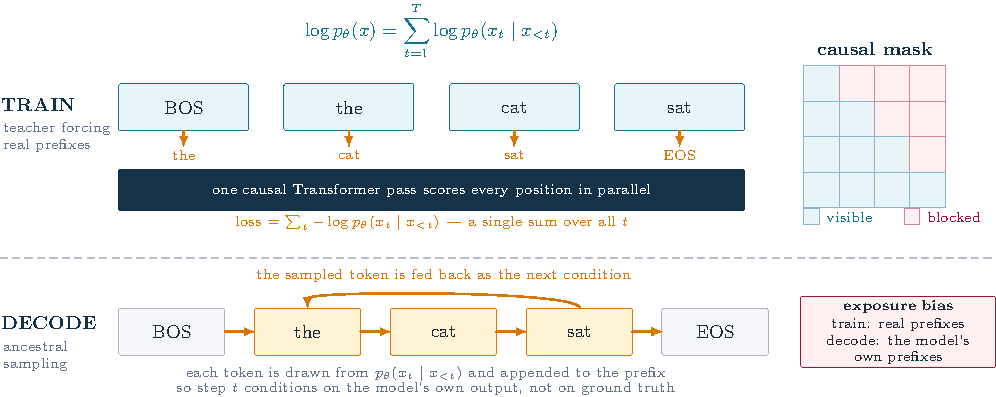
\includegraphics[width=\textwidth]{autoregressive_train_decode.pdf}
\caption{同一个自回归分解有两种计算组织。训练用真实前缀和因果 mask，在一次矩阵前向中并行监督所有位置；生成把刚采到的 token 追加到前缀，因而必须串行推进。}
\label{fig:autoregressive}
\end{figure}

\section{变分自编码器：潜变量与后验推断}

\subsection{潜变量模型与编码、解码}

图像中的姿态、风格或物理构型中的集体坐标，往往比原始数据更低维。VAE 先假设潜变量 \(z\) 的先验，以及给定 \(z\) 后观测 \(x\) 的条件分布；已有 \(x\) 时，再考虑如何推断未被观测的 \(z\)。常说的 encoder 和 decoder 是这两个概率计算方向的神经网络实现名称，出发点仍是潜变量模型与后验推断。

VAE 先假定数据 \(x\) 是由一个低维潜变量 \(z\) 生成的；其核心是把不可直接计算的后验推断改写成可优化的变分下界~\cite{kingma2013vae,rezende2014stochastic}。最常用的模型写成
\begin{equation}
 p_\theta(x,z)=p(z)p_\theta(x\mid z),\qquad
 p_\theta(x)=\int p(z)p_\theta(x\mid z)\,dz,
\end{equation}
其中 \(p(z)=\mathcal N(0,I)\) 是容易采样的先验，\(p_\theta(x\mid z)\) 是观测的条件分布。称作 decoder 的神经网络接收具体的 \(z\)，输出该分布的参数 \(\eta_\theta(z)\)。生成新数据依次需要采样 \(z\sim p(z)\)、计算 \(\eta_\theta(z)\)、再采样 \(x\sim p_\theta(\cdot\mid z)\)；困难在于训练时的边缘似然要对所有可能的 \(z\) 积分。

\subsection{变分下界与重构目标}

如果 decoder 是非线性神经网络，这个积分通常没有解析解，直接最大化 \(\log p_\theta(x)\) 也不能直接得到可反向传播的有限计算图。VAE 引入 encoder \(q_\phi(z\mid x)\) 作为真实后验 \(p_\theta(z\mid x)\) 的可计算近似。常见实现用一个共享的 encoder 主干和两个输出头产生 \(\mu_\phi(x)\) 与 \(\log\sigma_\phi^2(x)\)，定义 \(q_\phi(z\mid x)=\mathcal N\!\left(\mu_\phi(x),\operatorname{diag}\sigma_\phi^2(x)\right)\)。这个高斯分布描述的是给定 \(x\) 后潜变量 \(z\) 的近似后验；decoder 的观测分布 \(p_\theta(x\mid z)\) 则按数据类型选择。训练使用证据下界（Evidence Lower Bound，ELBO），“证据”指观测数据的边缘概率：
\begin{equation}
\begin{aligned}
 \mathcal L_{\mathrm{ELBO}}(x)
 &=\E_{q_\phi(z\mid x)}[\log p_\theta(x,z)-\log q_\phi(z\mid x)]\\
 &=\E_{q_\phi(z\mid x)}[\log p_\theta(x\mid z)]-\KL(q_\phi(z\mid x)\Vert p(z)).
\end{aligned}
\end{equation}
\Needspace{6\baselineskip}
这个目标为何是 \(\log p_\theta(x)\) 的下界？固定模型参数 \(\theta\) 和观测 \(x\)，把 Bayes 公式 \(p_\theta(z\mid x)=p_\theta(x,z)/p_\theta(x)\) 代入并整理，得到
\begin{equation}
\begin{aligned}
 \log p_\theta(x)-\mathcal L_{\mathrm{ELBO}}(x)
 &=\E_{q_\phi(z\mid x)}[\log q_\phi(z\mid x)-\log p_\theta(z\mid x)]\\
 &=\KL(q_\phi(z\mid x)\Vert p_\theta(z\mid x))\geq0.
\end{aligned}
\end{equation}
后验 KL 非负，所以 ELBO 不超过真实对数似然；当 \(q_\phi(z\mid x)=p_\theta(z\mid x)\) 时，两者相等。这个衡量下界松紧的后验 KL，与 ELBO 内部约束 \(q_\phi(z\mid x)\) 接近先验 \(p(z)\) 的 KL 是两个不同的量。真实后验通常也难以逐点计算，因此训练时优化可计算的 ELBO。最大化 ELBO 同时提高 decoder 条件分布对观测 \(x\) 的对数似然，并让 encoder 给出的潜变量分布接近可采样的先验。

第一项 \(\E_q[\log p_\theta(x\mid z)]\) 常叫重构项，实际计算的是已观测到的 \(x\) 在 decoder 所给条件分布下的对数概率。把网络输出的 \(\eta_\theta(z)\) 可视化时，通常得到一幅概率图或均值图；实际样本需另从分布抽取。这一项的具体形式由观测分布决定；选用 Bernoulli 或固定方差高斯分布时，会分别得到交叉熵或均方误差。对于二值数据 \(x\in\{0,1\}^D\)，经典例子让 decoder 输出每一位取 \(1\) 的概率 \(\pi_{\theta,j}(z)\)，并采用给定 \(z\) 后逐位独立的 Bernoulli 观测分布：
\begin{equation}
 p_\theta(x\mid z)=\prod_{j=1}^{D}\pi_{\theta,j}(z)^{x_j}\bigl[1-\pi_{\theta,j}(z)\bigr]^{1-x_j}.
\end{equation}
此时 \(-\log p_\theta(x\mid z)\) 正是逐位 binary cross-entropy；逐位独立只针对给定 \(z\) 的条件分布，边缘分布 \(p_\theta(x)\) 仍可有位与位之间的相关性。对于连续数据，另一种选择是高斯 decoder \(p_\theta(x\mid z)=\mathcal N(\mu_\theta(z),\sigma_x^2I)\)：固定方差时，负重构对数似然等于常数加 \(\|x-\mu_\theta(z)\|^2/(2\sigma_x^2)\)。第二项是 rate 或正则项，要求每个样本的编码分布不要随意偏离 \(p(z)\)，否则从先验采样出来的潜变量无法覆盖训练时的编码区域。

\subsection{重参数化与实际训练}

训练一个 minibatch 时，encoder 输出 \(\mu_\phi(x)\) 和 \(\log\sigma_\phi^2(x)\)，使用
\begin{equation}
 z=\mu_\phi(x)+\sigma_\phi(x)\odot\epsilon,\qquad
 \epsilon\sim\mathcal N(0,I),
\end{equation}
生成一个或少数几个 Monte Carlo 潜变量样本，再送入 decoder。对一个固定的训练样本 \(x\)，用 \(K\) 个独立潜变量样本估计负 ELBO：
\begin{equation}
\begin{aligned}
 \widehat{\mathcal J}_{\mathrm{VAE}}(x)
 &=-\frac{1}{K}\sum_{k=1}^{K}\log p_\theta(x\mid z^{(k)})
 +\KL(q_\phi(z\mid x)\Vert p(z)),\\
 &\hspace{9mm}z^{(k)}\sim q_\phi(\cdot\mid x).
\end{aligned}
\label{eq:vae-mc-loss}
\end{equation}
数据集的损失再对观测 \(x^{(i)}\) 取平均，实践中常取 \(K=1\)。这里每次都用同一个观测 \(x\) 评价 \(\log p_\theta(x\mid z^{(k)})\)，训练重构项时不需要从 decoder 再抽一个 \(x\)。若 \(q_\phi(z\mid x)\) 是对角高斯，KL 项可以精确计算：
\begin{equation}
 \KL\!\left(\mathcal N(\mu,\operatorname{diag}\sigma^2)\Vert\mathcal N(0,I)\right)
 =\frac12\sum_j\left(\mu_j^2+\sigma_j^2-\log\sigma_j^2-1\right).
\end{equation}
这里需要更新的是抽样分布 \(q_\phi(z\mid x)\) 的参数 \(\phi\)，因此使用第 \ref{sec:gradient-estimator-map} 节的重参数化路径。它把随机变量改写为与 \(\phi\) 无关的 \(\epsilon\)，随机性本身保留在 \(\epsilon\) 中，而 \(z\) 对 \(\mu_\phi,\sigma_\phi\) 变成可微的；梯度可以沿 \(x\to(\mu,\sigma)\to z\to\) decoder 反向传播。重构项对 decoder 参数 \(\theta\) 的梯度则是在抽到的 \(z\) 上直接求 \(\nabla_\theta\log p_\theta(x\mid z)\)。图 \ref{fig:vae-network} 把这一步训练画成网络：\(x\) 经 encoder 得到 \(\mu_\phi(x)\) 与 \(\sigma_\phi(x)\)，加入 \(\epsilon\) 抽出 \(z\)，decoder 再把 \(z\) 变回与 \(x\) 同形的 \(\hat x\)；\(\hat x\) 与 \(x\) 比较给出重构损失，\(\mu_\phi,\sigma_\phi\) 与先验比较给出 KL 损失。

\begin{figure}[H]
\centering
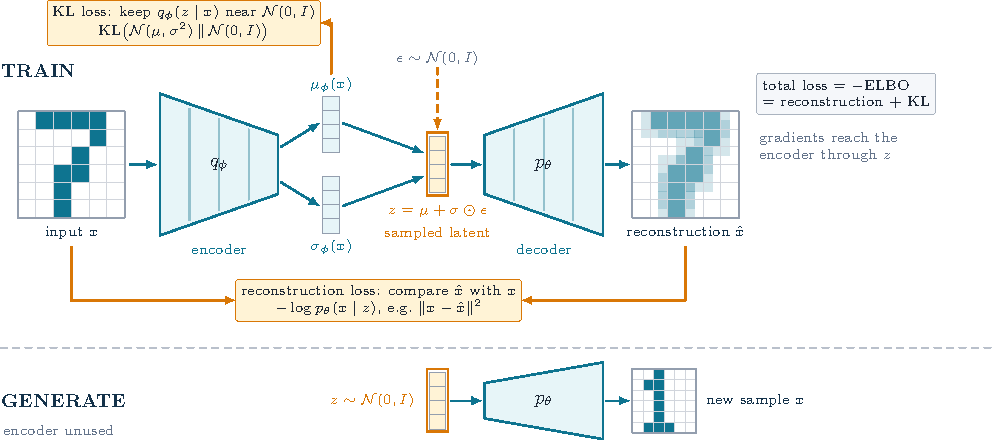
\includegraphics[width=\textwidth]{vae_network.pdf}
\caption{VAE 的网络结构。训练时，encoder 把输入 \(x\) 压缩为 \(q_\phi(z\mid x)\) 的参数 \(\mu_\phi(x),\sigma_\phi(x)\)，由 \(z=\mu+\sigma\odot\epsilon\) 抽出潜变量，decoder 把 \(z\) 展开为重构 \(\hat x\)，即 \(p_\theta(x\mid z)\) 的均值或概率图。重构损失 \(-\log p_\theta(x\mid z)\) 比较 \(\hat x\) 与 \(x\)，KL 损失约束编码分布接近 \(\mathcal N(0,I)\)，两者之和为负 ELBO。生成时不用 encoder，从先验抽 \(z\) 后只运行 decoder。各量之间的概率关系见图 \ref{fig:vae-architecture}。}
\label{fig:vae-network}
\end{figure}

\subsection{生成、重构与后验坍塌}

VAE 的推理有两种含义。生成新样本时从 \(p(z)\) 采样，运行 decoder 得到 \(p_\theta(x\mid z)\) 的参数，再从中采样 \(x\)；分析已有 \(x\) 时运行 encoder 得到 \(q_\phi(z\mid x)\)，可从中采样 \(z\)，再查看 decoder 给出的观测分布。所谓“重构图”通常显示该分布的均值或概率；随机样本需另从该分布抽取。训练复杂度主要是一次 encoder、一次 decoder 和少量潜变量样本，通常不随数据维度做高维积分；建模困难则来自 ELBO 松弛、先验与真实聚合后验不匹配，以及强 decoder 可能不使用潜变量。当 \(q_\phi(z\mid x)\approx p(z)\) 且每个潜变量维度的 KL 接近零时，就出现 posterior collapse；这时观测似然可能仍然很好，但 \(z\) 已经不携带样本特有信息。可以在训练初期减弱 KL 惩罚、随后逐步恢复，让编码器先学会携带样本信息；也可以限制解码器能力，降低其绕过潜变量解释数据的倾向~\cite{bowman2016generating}。

\begin{figure}[H]
\centering
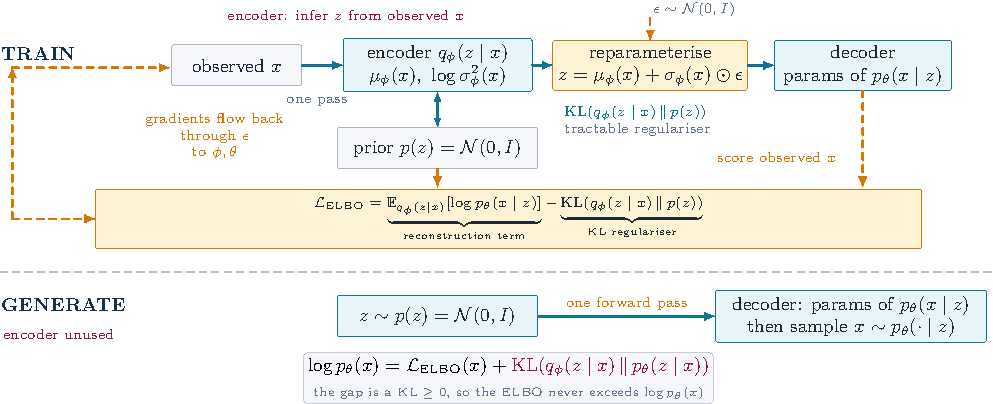
\includegraphics[width=\textwidth]{vae_architecture.pdf}
\caption{VAE 的训练与生成路径。左侧训练路径使用 encoder 得到 \(q_\phi(z\mid x)\)，随机性经重参数化 \(z=\mu+\sigma\odot\epsilon\) 引入，使梯度可以沿采样路径回传到 encoder；ELBO 的第一项是在 decoder 给出的条件分布下评价已观测 \(x\) 的对数概率，再减去 \(\KL(q_\phi(z\mid x)\Vert p(z))\)。右侧无条件生成路径从先验 \(p(z)=\mathcal N(0,I)\) 采样 \(z\)，由 decoder 输出观测分布 \(p_\theta(x\mid z)\) 的参数，再从中采样 \(x\)。ELBO 与真实 \(\log p_\theta(x)\) 之间的间隙正是 \(\KL(q_\phi(z\mid x)\Vert p_\theta(z\mid x))\)。}
\label{fig:vae-architecture}
\end{figure}

\subsection{离散潜变量：VQ-VAE}
\label{sec:vector-quantized-latents}

前面的高斯 VAE 用连续向量表示潜变量，但图像、语音和视频也可以先压缩成有限词表中的编号，再用离散序列模型学习这些编号的分布。例如，把一张图像编码成较小的二维编号网格，既能避开逐像素生成的长序列，又能把生成问题交给自回归 Transformer。向量量化变分自编码器（Vector-Quantized Variational Autoencoder，VQ-VAE）提供了这种从连续数据到离散潜变量的接口~\cite{vandenOord2017vqvae}。

设编码器在位置 \(i\) 输出 \(z_{e,i}(x)\in\R^d\)，可学习的码本为 \(\mathcal C=\{e_1,\ldots,e_M\}\subset\R^d\)。量化器选出最近的码字，用它代替编码器输出送入解码器：
\begin{equation}
 k_i(x)=\argmin_{1\leq j\leq M}\|z_{e,i}(x)-e_j\|_2^2,
 \qquad z_{q,i}(x)=e_{k_i(x)}.
 \label{eq:vq-lookup}
\end{equation}
例如，图像经过下采样编码器后得到 \(H'\times W'\) 个向量，每个位置执行一次式 \eqref{eq:vq-lookup}，便得到同样大小的整数索引网格 \((k_i)\)。每个整数 \(k_i\) 指向码本中的一个向量 \(e_{k_i}\)；把取出的向量按原来的空间位置排列，解码器便可据此重构图像。

训练的难点在于最近邻选择。只要 \(z_{e,i}\) 没有越过两个码字的分界面，\(z_{q,i}\) 就保持不变，因此量化映射对 \(z_{e,i}\) 的真实导数几乎处处为零，在分界面上不可导。VQ-VAE 采用直通估计（Straight-Through Estimator，STE）：用 \(\perp(u)\) 表示停止梯度操作，它在前向计算时等于 \(u\)，反向计算时对 \(u\) 的导数记为零。令
\begin{equation}
 \widetilde z_{q,i}=z_{e,i}+\perp(z_{q,i}-z_{e,i}).
 \label{eq:vq-straight-through}
\end{equation}
前向计算时 \(\widetilde z_{q,i}=z_{q,i}\)，解码器看到的仍是离散码字；反向计算时却规定 \(\partial\widetilde z_{q,i}/\partial z_{e,i}=I\)，把重构损失对解码器输入的梯度直接传给编码器。即使量化结果在一个邻域内完全不变，这个规则仍按单位导数回传。确定性的最近邻选择也没有可直接代入 score-function 公式的随机类别抽样分布。STE 是有意替换导数的工程折中，能帮助训练。

梯度直接传给编码器还不足以训练码本，因为式 \eqref{eq:vq-straight-through} 中的重构项不会沿这条路径更新 \(e_{k_i}\)。码本里的候选向量 \(e_1,\ldots,e_M\) 本身也是可训练参数；一种常用目标为
\begin{equation}
\begin{aligned}
 \mathcal J_{\mathrm{VQ}}(x)
 ={}&-\log p_\theta(x\mid\widetilde z_q)
 +\sum_i\|\perp(z_{e,i})-e_{k_i}\|_2^2\\
 &+\beta\sum_i\|z_{e,i}-\perp(e_{k_i})\|_2^2.
\end{aligned}
\label{eq:vq-loss}
\end{equation}
第一项更新解码器，并通过直通梯度更新编码器；第二项只更新本次被选中的码本向量，把它们拉向对应的编码器输出；第三项称为 commitment loss，只更新编码器，让输出靠近所选码字，\(\beta>0\) 控制其强度。码本向量也可以用编码器输出的移动平均更新。整数索引 \(k_i\) 不直接参与梯度更新，但编码器和码本向量改变后，下一次前向传播选中的索引可能随之改变。

离散变量也可以有 KL 散度：若 \(q_j,p_j\) 是两组类别概率，则 \(\KL(q\Vert p)=\sum_j q_j\log(q_j/p_j)\)。但这里的最近邻选择给出确定性的后验 \(q(k_i\mid x)\)：一个编号的概率为 1，其余为 0。若第一阶段暂取均匀先验 \(p(k_i)=1/M\)，则每个位置的 \(\KL(q(k_i\mid x)\Vert p(k_i))=\log M\) 是常数，不提供训练梯度。式 \eqref{eq:vq-loss} 后两项约束的是编码器输出与所选码字之间的距离，作用不同于高斯 VAE 中匹配后验与先验的 KL 项。

式 \eqref{eq:vq-loss} 的训练始终从真实图像 \(x\) 出发：编码器为各位置选出索引 \(k_i(x)\)，解码器利用对应的码本向量重构这张图像。若要不输入图像、从零生成新图像，就不能依靠编码器提供索引；此时还需要一个模型来决定每个位置该选哪个编号，以及不同位置的编号如何搭配。

为此，先用训练好的编码器把训练集中的每张图像变成索引网格，再按固定顺序读成序列。例如，\(2\times2\) 的网格 \(\bigl(\begin{smallmatrix}7&42\\3&19\end{smallmatrix}\bigr)\) 按行读成 \((7,42,3,19)\)。用这些真实图像产生的序列训练自回归 Transformer：给定前面的编号，预测下一个编号，并用真实编号计算交叉熵。这个索引序列的概率模型记为 \(p_\psi(k_1,\ldots,k_N)\)，其中 \(N=H'W'\)。生成时依次采样 \(N\) 个编号，按原顺序排回网格，把每个编号 \(k_i\) 换成码本向量 \(e_{k_i}\)，最后由已训练的解码器生成图像。

\Needspace{8\baselineskip}
\section{可逆流、对抗生成与能量模型}

\subsection{Normalizing Flow}

前面的高斯 VAE 需要对潜变量积分，使边缘似然难以精确计算。如果把数据与基分布之间的映射限制为同维、可逆的变换，就可以逐点追踪概率密度如何变化，并通过逆变换直接生成样本。这是下面可逆流模型的出发点。

Normalizing Flow 是一串可逆、可微的变换~\cite{papamakarios2021normalizing}。令 \(x\) 是数据空间中的样本，\(z=f_\theta(x)\) 是它在简单基分布中的坐标，例如 \(p_Z(z)=\mathcal N(0,I)\)。变量变换公式为
\begin{equation}
 \log p_X(x)=\log p_Z(f_\theta(x))+\log\left|\det\frac{\partial f_\theta(x)}{\partial x}\right|.
\end{equation}
如果直接用任意神经网络表示 \(f_\theta\)，它虽然可能有很强的表达能力，但既不一定可逆，也需要计算一个 \(d\times d\) Jacobian 的行列式。RealNVP 用 affine coupling layer 解决这两个问题~\cite{dinh2016density}。把输入按 mask 分成 \(x=(x_a,x_b)\)，第一部分直接复制，第二部分由第一部分产生 scale 和 shift：
\begin{align}
 z_a&=x_a,\\
 z_b&=x_b\odot\exp s_\theta(x_a)+t_\theta(x_a).
\end{align}
这里 \(s_\theta,t_\theta\) 可以是普通的卷积网络或多层感知机，它们本身不需要可逆；可逆性来自 \(x_b\) 只做逐元素的仿射变换。逆变换可以显式写出：
\begin{equation}
 x_a=z_a,\qquad
 x_b=\left(z_b-t_\theta(z_a)\right)\odot\exp[-s_\theta(z_a)].
\end{equation}

它能快速计算 Jacobian，是因为矩阵具有块三角结构：
\begin{equation}
 \frac{\partial z}{\partial x}
 =
 \begin{bmatrix}
 I & 0\\
 \frac{\partial z_b}{\partial x_a}
 & \operatorname{diag}\!\left(\exp s_\theta(x_a)\right)
 \end{bmatrix},
 \qquad
 \log|\det J|=\sum_j s_{\theta,j}(x_a).
\end{equation}
行列式只等于对角线元素的乘积，不需要对完整 Jacobian 做 \(O(d^3)\) 的通用行列式计算；在多层 coupling layer 中，log-determinant 只是每层 scale 输出的求和。不同层交替 mask，使前一层没有改变的 \(x_a\) 在下一层成为被变换的部分，否则模型会永久保留一半输入不变。

Flow 的训练目标是真实数据的精确负对数似然：
\begin{equation}
 \mathcal L_{\mathrm{Flow}}
 =-\frac1N\sum_i\left[
 \log p_Z(f_\theta(x^{(i)}))
 +\log|\det J_{f_\theta}(x^{(i)})|
 \right].
\end{equation}
训练时把数据 \(x\) 经过各层正向变换得到 \(z\)，基分布 log-density 和每层 log-determinant 都能反向传播到 \(s_\theta,t_\theta\)。前向训练不需要从模型中抽样，也没有 VAE 那样的潜变量积分；生成时才从 \(z\sim p_Z\) 随机采样，再按相反顺序运行显式逆变换得到 \(x\)。因此 Flow 同时有精确 likelihood、可逆编码和直接采样，但它必须牺牲一部分任意神经网络的自由度来保证可逆性；高维数据的多尺度分解、边界处理、scale 爆炸和层数带来的逆向成本都是主要架构难点。

\begin{figure}[H]
\centering
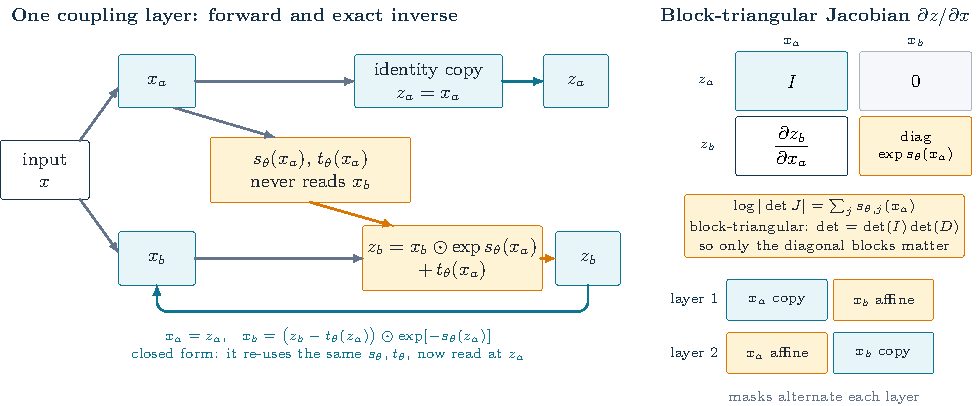
\includegraphics[width=\textwidth]{realnvp_architecture.pdf}
\caption{RealNVP coupling layer 的正向与逆向计算。复制分支把 \(x_a\) 原样送出，scale/shift 网络只读取 \(x_a\) 并产生逐元素仿射参数，因此 \(x_b\) 的变换是逐元素的，整个映射可以显式求逆。右侧的块三角 Jacobian 说明行列式只等于对角块 \(\operatorname{diag}(\exp s_\theta(x_a))\) 的乘积，log-determinant 退化为 \(\sum_j s_{\theta,j}(x_a)\)，无需 \(O(d^3)\) 的通用行列式计算。相邻层交换 mask 划分，避免一半输入始终不变。}
\label{fig:realnvp-architecture}
\end{figure}

\subsection{连续归一化流：神经常微分方程（Neural ODE）与密度演化}
\label{sec:cnf}

RealNVP 通过有限层变换逐层累加 log-determinant。另一种做法是把层间更新写成 \(x_{k+1}=x_k+\Delta r\,v_\theta(x_k,r_k)\)，并在 \(\Delta r\to0\) 时用连续时间 \(r\in[0,1]\) 描述从基分布到数据分布的运动：
\begin{equation}
 \frac{dx_r}{dr}=v_\theta(x_r,r),\qquad x_{r=0}=z\sim p_0.
 \label{eq:cnf-ode}
\end{equation}
用神经网络表示微分方程右侧的速度场，并通过数值求解器积分得到 \(x_1\)，这就是 Neural ODE 的基本计算路径~\cite{chen2018neuralode}。训练时还要计算损失对 \(\theta\) 的梯度：可以让自动微分穿过数值积分的各步，也可以使用伴随灵敏度方程。因而 Neural ODE 把“解微分方程得到输出”与“梯度能穿过求解过程”放在同一模型中；积分步数和梯度计算方式决定实际训练成本。

当这条 ODE 用于概率建模时，还需要追踪运动中的密度，这样的模型称为连续归一化流~\cite{chen2018neuralode,grathwohl2019ffjord}。样本沿式 \eqref{eq:cnf-ode} 运动时，概率质量守恒给出连续性方程 \(\partial_r p_r=-\nabla\cdot(p_rv_\theta)\)。沿单条轨迹使用链式法则，得到瞬时变量变换公式
\begin{equation}
 \frac{d}{dr}\log p_r(x_r)
 =-\nabla\cdot v_\theta(x_r,r)
 =-\operatorname{tr}\!\left(\frac{\partial v_\theta}{\partial x}(x_r,r)\right).
 \label{eq:cnf-density}
\end{equation}
因此，从 \(z=x_{r=0}\) 积分到 \(x=x_{r=1}\) 时，\(\log p_1(x)=\log p_0(z)-\int_0^1\nabla\cdot v_\theta(x_r,r)\,dr\)。生成只需从 \(p_0\) 抽样并向前积分；评价给定数据 \(x\) 的密度则从 \(x_{r=1}=x\) 反向积分到 \(z\)，同时累积散度。与有限层变换中的 Jacobian 行列式相比，连续时间的局部体积变化由迹表示：\(\log\det(I+\Delta r J)=\Delta r\operatorname{tr}J+O(\Delta r^2)\)。速度网络因而可以采用较自由的结构；在保证 ODE 解唯一性的常规条件下，正向与反向积分给出互逆映射。

若直接用 \(-\log p_1(x)\) 训练 CNF，每次更新都要数值求解状态和散度的积分，再把梯度传回速度网络。迹的计算在高维时仍有代价，可用迹估计等方法处理；数值求解精度也影响最终的密度值。后面的 Flow Matching 将保留同一个生成 ODE，改用已知概率路径的速度作为训练标签。

\subsection{生成对抗网络}
\label{sec:gan}

如果任务重点是快速产生逼真的样本，可以放松对显式似然的要求，让一个辅助网络判断生成结果与真实数据的差别，再把这种反馈传给生成器。这样生成网络能采用更自由的结构，训练则需要协调两个网络。

GAN 用生成器 \(G_\theta(z)\) 把简单噪声 \(z\sim p_Z\) 推送成样本，用判别器 \(D_\phi(x)\in(0,1)\) 判断输入来自真实数据还是生成器~\cite{goodfellow2014gan}。原始 minimax 目标是
\begin{equation}
 \min_\theta\max_\phi V(D_\phi,G_\theta)
 =\E_{x\sim p_{\mathrm{data}}}\log D_\phi(x)
 +\E_{z\sim p_Z}\log\left[1-D_\phi(G_\theta(z))\right].
\end{equation}
对固定的生成分布 \(p_g\)，若判别器有无限容量且达到最优，它在每个 \(x\) 上的解为
\begin{equation}
 D^*(x)=\frac{p_{\mathrm{data}}(x)}
 {p_{\mathrm{data}}(x)+p_g(x)}.
\end{equation}
把 \(D^*\) 代回目标后，生成器的目标可写成 Jensen--Shannon 散度（Jensen--Shannon Divergence，JSD）：
\begin{equation}
 V(D^*,G)=-\log 4+
 2\,\operatorname{JSD}\!\left(p_{\mathrm{data}}\Vert p_g\right),
\end{equation}
JSD 是对称散度，其值在两个分布一致时为零。理想 Nash equilibrium 的含义是 \(p_g=p_{\mathrm{data}}\)，此时 \(D^*(x)=1/2\)，判别器无法从样本判断真假，生成器也没有方向继续改善；这个平衡在无限数据、无限模型容量和全局最优的设定下成立，有限网络的交替训练是它的近似。

实践中每一步先固定 \(G\) 更新判别器，再固定 \(D\) 更新生成器。原始生成器损失 \(\E_z\log[1-D(G(z))]\) 在判别器很强时容易梯度饱和：若生成样本很容易被识别，\(D(G(z))\approx0\)，判别器末端 sigmoid 已落在接近水平的区域，链式法则传回生成器的梯度因而接近零。这里的“饱和”指的是原始生成器目标在当前参数区间几乎不给出可用的改进方向。因此交替训练时常用 non-saturating loss
\begin{equation}
 \mathcal L_G^{\mathrm{non\text{-}saturating}}=-\E_{z\sim p_Z}\log D_\phi(G_\theta(z)).
\end{equation}
它与 minimax 目标拥有相同的理想平衡点，区别在于梯度从哪个方向进入。原始生成器目标对生成器参数的梯度是
\begin{equation}
 \nabla_\theta\E_z\log[1-D(G(z))]=-\E_z\frac{\nabla_\theta D(G(z))}{1-D(G(z))},
\end{equation}
当 \(D(G(z))\approx0\) 时分母接近 \(1\)，梯度量级较小；而 non-saturating 损失的梯度是
\begin{equation}
 \nabla_\theta\left[-\E_z\log D(G(z))\right]=-\E_z\frac{\nabla_\theta D(G(z))}{D(G(z))},
\end{equation}
此时分母接近 \(0\)，梯度被放大。也就是说，判别器越确信生成样本是假的，non-saturating 损失给出的更新方向反而越强，而原始 minimax 形式的生成器梯度则趋于消失。代价是 non-saturating 损失在生成器已经能骗过判别器时权重变小，学习信号随之减弱；两者的平衡点相同，梯度在训练不同阶段的有效性不同。

GAN 的生成器需要对自己产生的样本求导：噪声 \(z\sim p_Z\) 与 \(\theta\) 无关，给定 \(z\) 后，梯度沿 \(z\to G_\theta(z)\to D_\phi(G_\theta(z))\) 回传。这是第 \ref{sec:gradient-estimator-map} 节的路径梯度；由于输入噪声已经固定分布，不需要再做 VAE 式的重参数化。GAN 不显式计算 \(p_g(x)\) 或 likelihood，推理时只需一次 \(G_\theta\) 前向传播，代价低；训练却是非凸的双层博弈，判别器过强、梯度不平衡和 mode collapse 会使生成器只覆盖少数容易骗过判别器的模式。图 \ref{fig:gan-architecture} 画出两步交替更新的数据流和梯度路径：判别器步只更新 \(\phi\)；生成器步固定 \(D_\phi\)，梯度穿过判别器和生成样本回到 \(G_\theta\)。

\begin{figure}[ht]
\centering
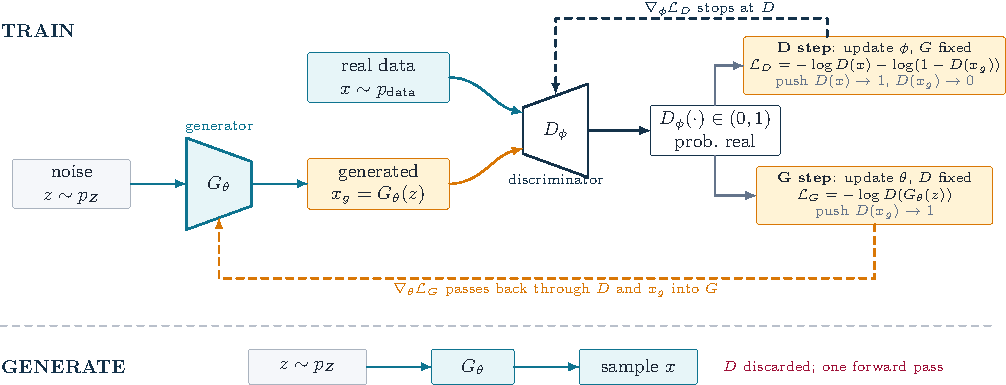
\includegraphics[width=\textwidth]{gan_architecture.pdf}
\caption{GAN 的网络结构与交替训练。生成器 \(G_\theta\) 把噪声 \(z\) 映成样本 \(x_g\)，判别器 \(D_\phi\) 对真实样本和生成样本输出“为真”的概率。判别器步固定 \(G\)，用 \(\mathcal L_D\) 更新 \(\phi\)；生成器步固定 \(D\)，用 non-saturating 损失 \(\mathcal L_G\) 更新 \(\theta\)，梯度经 \(D\) 与 \(x_g\) 回到 \(G\)。生成时丢弃判别器，只做一次生成器前向。}
\label{fig:gan-architecture}
\end{figure}

\begin{figure}[ht]
\centering
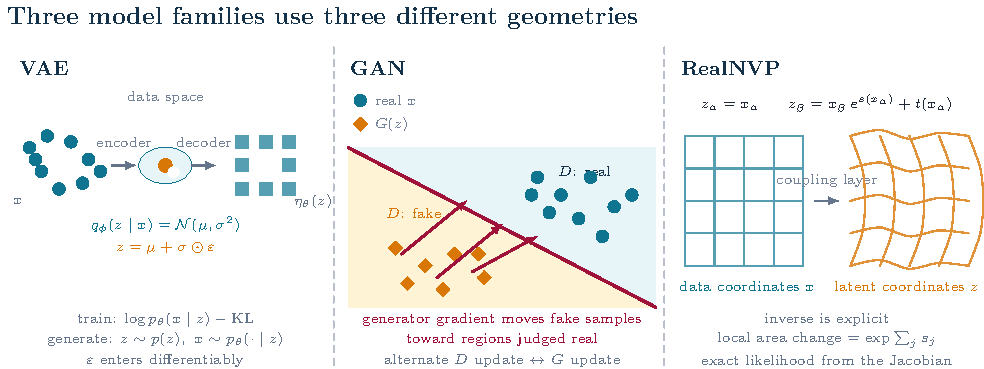
\includegraphics[width=\textwidth]{vae_gan_realnvp_networks.pdf}
\caption{VAE、GAN 和 RealNVP 的神经网络与梯度路径对照。VAE 面板的像素网格表示 decoder 输出的观测分布参数 \(\eta_\theta(z)\)，具体样本还需从该分布抽取；VAE 的随机性通过 \(\epsilon\) 进入可微重参数化。GAN 的生成器通过判别器损失获得梯度；RealNVP 通过耦合层的显式逆变换和三角 Jacobian 保持可逆。}
\label{fig:generative-network-comparison}
\end{figure}

\subsection{核匹配与量子线路 Born machine}

GAN 说明，即使难以逐点计算 \(p_\theta(x)\)，只要能够从模型采样，仍可用真实样本和生成样本训练模型。另一条训练路径是直接比较两组样本的统计量。经典的生成矩匹配网络（Generative Moment Matching Network，GMMN）使用最大均值差异（Maximum Mean Discrepancy，MMD）作为生成损失~\cite{li2015gmmn,gretton2012kernel}。

给定正定核函数 \(k(x,y)=\langle\phi(x),\phi(y)\rangle_{\mathcal H_k}\)，核技巧允许我们通过样本对上的 \(k(x,y)\) 比较特征均值，而不必显式构造可能无限维的特征映射 \(\phi\)。其平方损失为
\begin{align}
 \mathcal L_{\mathrm{MMD}}(\theta)
 &=\left\|\E_{x\sim p_{\mathrm{data}}}\phi(x)-\E_{y\sim p_\theta}\phi(y)\right\|_{\mathcal H_k}^{2}\notag\\
 &=\E_{x,x'\sim p_{\mathrm{data}}}k(x,x')
 +\E_{y,y'\sim p_\theta}k(y,y')
 -2\E_{x\sim p_{\mathrm{data}},\,y\sim p_\theta}k(x,y).
\end{align}
其中 \(x,x'\) 和 \(y,y'\) 分别是各自分布中的独立样本；三个期望都可以用两个样本批次中的样本对估计。例如，连续向量可用高斯核，比特串可用基于汉明距离的核；核的选择决定训练时关注哪些样本差别。对于能区分分布的特征核，理论上 \(\operatorname{MMD}(p,q)=0\) 当且仅当 \(p=q\)。

从“用测试函数区分两组样本”的角度看，MMD 可以直观地理解为一种限制了判别方式的 GAN：它把测试函数限制在预先选定的核函数空间的单位球内，取两组样本在这些函数上的最大期望差；GAN 则训练判别网络来学习区分特征。这个类比只说明训练信号的来源；原始 GAN 的目标对应理想条件下的 Jensen--Shannon 散度，MMD 则是核函数空间中的分布距离。固定核省去了交替优化，目标较直接；但在高维数据中，基于距离的核及其宽度未必反映有用的结构，过宽的核会抹平差别，过窄的核又可能让两组样本之间几乎没有训练信号。对大小为 \(B\) 的批次，直接计算经验 MMD 还需 \(O(B^2)\) 个样本对核值。GAN 的可学习判别器能够适应复杂特征，却引入博弈不稳定和模式缺失的风险；若让网络学习 MMD 所用的特征，也会重新引入类似的对抗优化~\cite{li2017mmdgan}。

量子线路 Born machine（Quantum Circuit Born Machine，QCBM）展示了用参数化量子线路构造生成器的方法~\cite{liu2018qcbm}。参数化线路 \(U_\theta\) 制备量子态，对 \(n\) 个量子比特测量即可得到比特串 \(x\in\{0,1\}^n\)，其概率由 Born 规则定义为
\begin{equation}
 p_\theta(x)=\left|\langle x|U_\theta|0^n\rangle\right|^2.
\end{equation}
采样只需运行并测量线路；要从有限测量次数高精度估计某个稀有比特串的相对概率则很昂贵。于是可以直接把真实比特串与测量结果放进上面的 MMD 损失，而不计算逐点似然。经典 GMMN 需要对生成样本上的核函数求导，可沿可微生成器使用第 \ref{sec:gradient-estimator-map} 节的路径梯度；QCBM 的离散测量结果没有这条梯度路径，训练常对可移位参数门使用参数移位规则，运行偏移参数的线路来估计损失梯度。因此“容易采样”解决了损失评估所需的模型样本，参数优化仍需多次线路运行。QCBM 是按 Born 规则定义分布，与下节按能量和配分函数定义分布的 Boltzmann machine 不同。

\subsection{能量模型与 MCMC}
\label{sec:ebm-mcmc}

有些任务很容易判断一个构型是否合理，却很难直接给出它的归一化概率。例如，物理哈密顿量能为每个构型计算能量，但平衡分布的配分函数需要遍历整个构型空间。能量模型沿用这一思路：先给样本打能量分数，再解决归一化与采样。

EBM（Energy-Based Model，能量模型）用一个能量函数 \(E_\theta(x)\) 规定一条未归一化密度：
\begin{equation}
 p_\theta(x)=Z_\theta^{-1}\exp[-E_\theta(x)],\qquad
 Z_\theta=\int\exp[-E_\theta(x)]\,dx.
\end{equation}
\(E_\theta\) 可以是任意标量函数，灵活度高于显式密度模型；物理中“能量越低概率越高”的先验也可以直接写进 \(E_\theta\)。代价全部落在配分函数 \(Z_\theta\) 上：它是对整个 \(x\) 空间的积分，除极少数特例都无法解析计算，而 \(Z_\theta\) 同时出现在归一化、采样和训练梯度三个地方。训练梯度可以把它约掉，采样也能在不知道 \(Z_\theta\) 的情况下进行。

\textbf{最大似然的参数梯度。}把 \(\log p_\theta(x)=-E_\theta(x)-\log Z_\theta\) 对 \(\theta\) 求导，第一项直接给出 \(-\nabla_\theta E_\theta(x)\)，第二项需要处理 \(Z_\theta\) 对参数的依赖。关键事实是：虽然 \(Z_\theta\) 本身算不出来，它的对数梯度却可以写成对模型分布取期望的形式，
\begin{align}
 \nabla_\theta\log Z_\theta
 &=\frac{1}{Z_\theta}\nabla_\theta\int\exp[-E_\theta(x)]\,dx
 =\frac{1}{Z_\theta}\int-\nabla_\theta E_\theta(x)\exp[-E_\theta(x)]\,dx\notag\\
 &=-\int p_\theta(x)\nabla_\theta E_\theta(x)\,dx
 =-\E_{p_\theta}[\nabla_\theta E_\theta(x)].
\end{align}
第二个等号把梯度移进积分，第三个等号把 \(\exp[-E_\theta]/Z_\theta\) 整体识别成 \(p_\theta(x)\)。右端不用显式求出 \(Z_\theta\)，但仍需得到服从模型分布的样本，才能估计这个期望。把两项合起来并对数据取期望，
\begin{equation}
 \nabla_\theta\mathcal L_{\mathrm{NLL}}
 =\underbrace{\E_{p_{\mathrm{data}}}[\nabla_\theta E_\theta(x)]}_{\text{positive phase}}
 -\underbrace{\E_{p_\theta}[\nabla_\theta E_\theta(x)]}_{\text{negative phase}}.
\end{equation}
第一项只在真实数据上求值，实现简单，作用是降低数据点的能量；第二项要求在模型自身分布 \(p_\theta\) 上取期望，无法解析计算，只能采样。正负相位的名称来自统计物理中玻尔兹曼机的用法：负相位是把已建立的“模型样本能量”推高，使得模型不能靠把所有能量都压低来退化解。所以 EBM 的训练困难不在梯度公式，而在于每一步参数更新前都要先运行一次采样。

第 \ref{sec:gradient-estimator-map} 节讨论了如何对参数化抽样目标求导；这里的模型期望已由 \(\nabla_\theta\log Z_\theta\) 的解析求导得到，MCMC 只负责取得负相位样本，不需要对马尔可夫链的抽样步骤求导。

\textbf{用 MCMC 采样负相位。}目标是构造一条马尔可夫链，使其平稳分布恰好是 \(p_\theta\)，从而在链运行足够久之后把它当作 \(p_\theta\) 的样本。

Metropolis--Hastings（MH）从当前状态 \(x\) 按提议分布 \(q(x'\mid x)\) 抽一个候选 \(x'\)。其接受概率为
\begin{equation}
 a(x'\mid x)=\min\left\{1,\ \frac{\tilde p_\theta(x')q(x\mid x')}{\tilde p_\theta(x)q(x'\mid x)}\right\}.
\end{equation}
这里 \(\tilde p_\theta(x)=\exp[-E_\theta(x)]\) 是未归一化密度。接受率只用到未归一化密度的比值，\(Z_\theta\) 在分子分母同时出现并约掉，这就是 MCMC 绕开配分函数的机制。可以验证该接受率满足细致平衡 \(\tilde p_\theta(x)q(x'\mid x)a(x'\mid x)=\tilde p_\theta(x')q(x\mid x')a(x\mid x')\)，对 \(x\) 积分即得 \(p_\theta\) 是平稳分布。

Gibbs sampling 是 MH 的一个特例：当某个变量的条件分布在其余变量给定时可以精确采样时，直接从这个条件分布抽新值，接受率恒等于 \(1\)。它在 EBM 上能否使用取决于能量函数的结构。下面的受限玻尔兹曼机（RBM, Restricted Boltzmann Machine）就是一个条件分布可以精确计算的特例，它的例子把上面的正相位、负相位和持续链落成可执行步骤。

Langevin dynamics 用能量梯度构造新的候选状态 \(x'\)，适用于 \(E_\theta\) 可微的连续变量。连续时间形式是
\begin{equation}
 dx=-\tfrac12\nabla_x E_\theta(x)\,dt+dW_t,
\end{equation}
其中 \(W_t\) 是标准布朗运动，增量 \(dW_t\) 在时长 \(dt\) 内的协方差为 \(I\,dt\)。把它按步长 \(\eta\) 离散，就得到正文使用的迭代
\begin{equation}
 x_{k+1}=x_k-\frac{\eta}{2}\nabla_x E_\theta(x_k)+\sqrt{\eta}\,\xi_k,\qquad \xi_k\sim\mathcal N(0,I),
 \label{eq:langevin-step}
\end{equation}
它由“沿能量梯度下坡”和“热噪声扩散”两部分组成，噪声使链有机会离开局部极小值。这样构造为什么正确，可以用 Fokker--Planck 方程验证：该随机微分方程对应的密度演化方程是
\(\partial_t p=\tfrac12\nabla\cdot\bigl(p\nabla E_\theta+\nabla p\bigr)\)，代入 \(p\propto\exp(-E_\theta)\) 后括号内两项恰好抵消，右端为零，因此 \(p_\theta\) 正是它的平稳分布。在常见的光滑性和稳定性条件下，这种离散化会产生随步长变化的平稳分布偏差：直接使用上式是不加校正的 Langevin 算法，步长有限时采样分布偏离 \(p_\theta\)。把 Langevin 提议放进上面的 MH 接受/拒绝步骤，偏差被消除，得到带 Metropolis 接受校正的 Langevin 算法；代价是每步要评估候选点的能量与梯度以计算接受率，而步长 \(\eta\) 的选取同时影响探索状态空间的速度与偏差大小。这解释了它与 MCMC 的关系：Langevin 动力学提供一种梯度引导的采样机制；有限步长时可用 MH 校正保持目标平稳分布，也可接受不校正的离散化偏差。

即使采样方法以 \(p_\theta\) 为平稳分布，有限步的链也未必已接近它。这里的 mixing（混合）指马尔可夫链忘记初值并在各个高概率模式之间按目标权重移动的速度；若链只在一个能量谷附近来回，即使步数很多，得到的仍是高度相关且有偏的负样本。

\textbf{负相位的两种近似。}精确估计负相位要求样本服从 \(p_\theta\)，而训练时每个 minibatch 都要重算一次负相位，等待链充分混合的代价过高。常见做法是接受一个有偏但便宜的估计。

CD-\(k\)（Contrastive Divergence，\(k\) 步对比散度）从真实数据点出发，只跑 \(k\) 步 Gibbs 或 Langevin，用短链终点作为负样本，\(k\) 在实践中常取 \(1\)。它的更新量是“数据点的能量梯度减短链终点的能量梯度”。起点在数据附近使链不必先 burn-in，代价是终点尚未收敛到 \(p_\theta\)，因此所得更新带有短链偏差，主要探测数据附近模型赋予过高概率的区域，属于局部近似，不能保证覆盖所有模式。

PCD（Persistent Contrastive Divergence，持续对比散度）把上一条链的终点保存下来，作为下一次参数更新时链的起点，从而不必每轮重新 burn-in。风险是参数在链还未平衡时已经改变，链追踪的是一个持续移动的分布；若能量面存在相距很远的模式，链可能长期停在其中一个模式，负样本的分布因此系统性偏离 \(p_\theta\)。实务中需要监控多链的能量、自相关时间和跨模式跃迁。

\begin{examplebox}[RBM：一个能看见 Gibbs 更新细节的 EBM]
RBM 把二值可见变量 \(v\) 和隐藏变量 \(h\) 的能量写成
\begin{equation}
E(v,h)=-a^\mathsf Tv-b^\mathsf Th-v^\mathsf TWh.
\end{equation}
“受限”表示同一层内没有连接，因此 \(p(h_j=1\mid v)=\sigma(b_j+W_{:j}^\mathsf Tv)\) 和 \(p(v_i=1\mid h)=\sigma(a_i+W_{i:}h)\) 都可并行采样。一次 PCD 更新就是：保存 \(v^-\)，交替采样 \(h^-\sim p(h\mid v^-)\)、\(v^-\sim p(v\mid h^-)\) 若干步，用数据对 \((v^+,h^+)\) 与模型对 \((v^-,h^-)\) 的相关量之差更新 \(W\)，再把新的 \(v^-\) 留给下一轮。这个例子把“负相位”“持续链”和“混合”落实成了可执行步骤。
\end{examplebox}

训练之外，推理时 EBM 同样没有闭式前向采样，生成一个样本仍需运行许多 MCMC 步，因此采样速度和跨模式移动能力是它的核心限制。

\textbf{用得分匹配替代负相位采样。}当数据连续、密度足够光滑时，可以学习密度在每个数据点附近如何变化。得分函数（score）定义为 \(s_\theta(x)=\nabla_x\log p_\theta(x)\)：它是一个与 \(x\) 同维的向量，指向局部对数密度上升最快的方向。对能量模型，\(s_\theta=-\nabla_xE_\theta\)，因为配分函数对输入 \(x\) 是常数。得分匹配（score matching）最初就是为未归一化密度提出的~\cite{hyvarinen2005score}；它希望最小化
\begin{equation}
 J(\theta)=\frac12\int p(x)\|s_\theta(x)-\nabla_x\log p(x)\|^2\,dx,
 \label{eq:score-matching-target}
\end{equation}
这里 \(p=p_{\mathrm{data}}\) 表示数据的光滑总体密度。真实 score 未知，但结论可以先说：经分部积分，这个目标只差一个常数地等于 \(\E_p[\tfrac12\|s_\theta\|^2+\nabla\cdot s_\theta]\)，只需在数据样本上计算模型 score 及其散度，既不需要真实 score，也不需要负样本。推导分三步。

首先展开平方，并把与 \(\theta\) 无关的真实 score 平方项记为常数 \(C\)：
\begin{align}
 J(\theta)&=\frac12\E_p\|s_\theta\|^2-\int p(x)s_\theta(x)\cdot\nabla\log p(x)\,dx+C\\
 &=\frac12\E_p\|s_\theta\|^2-\sum_{j=1}^{d}\int s_{\theta,j}(x)\,\partial_jp(x)\,dx+C.
\end{align}
第二步只用了 \(p\,\partial_j\log p=\partial_jp\)。对每个坐标做分部积分，若边界项消失（例如无穷远处 \(p\,s_{\theta,j}\) 足够快趋零），则
\begin{equation}
 \int s_{\theta,j}\,\partial_jp\,dx
 =-\int p\,\partial_js_{\theta,j}\,dx.
\end{equation}
最后代回，交叉项的负号变成正号，得到
\begin{equation}
 J(\theta)=\E_p\!\left[\frac12\|s_\theta(x)\|^2+\nabla\cdot s_\theta(x)\right]+C,
 \label{eq:score-matching-computable}
\end{equation}
其中散度 \(\nabla\cdot s_\theta=\sum_j\partial_js_{\theta,j}\)；若 \(s_\theta=\nabla\log p_\theta\)，它就是 \(\log p_\theta\) 对输入的 Hessian 矩阵的迹。对由标量能量 \(E_\theta\) 定义的模型，把 \(s_\theta=-\nabla_xE_\theta\) 代入，实际最小化的样本平均是
\begin{equation}
 \widehat J(\theta)=\frac1B\sum_{i=1}^{B}\left[\frac12\|\nabla_xE_\theta(x_i)\|^2-\operatorname{tr}\!\left(\nabla_x^2E_\theta(x_i)\right)\right],
 \label{eq:ebm-score-matching-batch}
\end{equation}
省去了与 \(\theta\) 无关的常数。每个 \(x_i\) 都来自真实数据 minibatch，不需要从当前能量模型采负样本。第一项先前向计算标量 \(E_\theta(x_i)\)，再用自动微分对输入 \(x_i\) 求梯度，并把各坐标的梯度平方相加。第二项是同一能量函数对输入的 Hessian 对角线之和；低维时可逐坐标对 \(\partial_{x_j}E_\theta\) 再求一次 \(\partial_{x_j}\)，高维时这样做要计算许多二阶导数。

\Needspace{13\baselineskip}
高维的一个实用近似是为每个样本抽取若干独立随机向量 \(v_k\)，使 \(\E[v_kv_k^\mathsf T]=I\)，例如每个分量独立取 \(+1\) 或 \(-1\)。利用随机迹估计，
\begin{equation}
 \operatorname{tr}(\nabla_x^2E_\theta(x_i))
 =\E_v\!\left[v^\mathsf T\nabla_x^2E_\theta(x_i)v\right]
 \approx\frac1K\sum_{k=1}^{K}v_k^\mathsf T\nabla_x^2E_\theta(x_i)v_k.
\end{equation}
实际计算无需存下整个 Hessian：先求 \(g(x)=\nabla_xE_\theta(x)\)，再对标量 \(g(x)\cdot v_k\) 关于 \(x\) 求梯度，便得到 Hessian--向量积 \(\nabla_x^2E_\theta(x)v_k\)。将这两项的 minibatch 均值对参数 \(\theta\) 反向传播时，必须保留输入导数的计算图。随机迹估计省去逐坐标计算，但有抽样方差；切片得分匹配还将第一项投影到随机方向，已被用于训练深度能量模型~\cite{song2020sliced}。这种训练避免了负相位 MCMC，却要求能量函数能对输入稳定求导；下一节把目标放到带噪密度上，用已知噪声构造去噪回归，从而避免显式计算散度。

\subsection{按权重采样：生成流网络}
\label{sec:gflownet}

EBM 把目标写成 \(p(x)\propto e^{-E(x)}\)，采样留给马尔可夫链。若这个未归一化目标已经由外部给出，还可以把“构造 \(x\)”的过程学成一个策略：训练完成后，从初始状态一路采样到终止状态，得到一个样本；样本出现的频率正比于 \(R(x)\)。这类模型叫生成流网络（Generative Flow Network，GFlowNet）~\cite{bengio2021gflownet}。

这里的 \(R\) 是未归一化权重，目标分布是 \(p(x)=R(x)/Z\)。取 \(R(x)=e^{-\beta E(x)}\) 就得到玻尔兹曼分布，温度由 \(\beta\) 控制；取 \(R(x)=\exp(r(x)/\tau)\) 就得到第一章的 KL 倾斜解。后文沿用 GFlowNet 文献的“奖励”一词，但它在数学上始终是这条权重。

设状态图是一个有向无环图，从初始状态 \(s_0\) 出发，每步选择一个动作转移到下一个状态，终止状态就是样本 \(x\)。前向策略 \(P_F(s'\mid s)\) 决定怎样构造；反向策略 \(P_B(s\mid s')\) 只在训练时用来计算回流。一条完整轨迹 \(\tau=(s_0,\ldots,s_n=x)\) 的前向概率和反向概率分别是
\begin{equation}
 P_F(\tau)=\prod_{t=0}^{n-1}P_F(s_{t+1}\mid s_t),\qquad
 P_B(\tau\mid x)=\prod_{t=1}^{n}P_B(s_{t-1}\mid s_t).
 \label{eq:gfn-path-prob}
\end{equation}
给定终止状态的未归一化目标 \(R(x)\ge0\)，训练要让 \(P_F\) 满足下面的轨迹平衡。

\(P_F\) 和 \(P_B\) 都是可学习的概率函数，通常共用一个状态编码器和两个输出头。给定状态 \(s\) 的编码向量，前向头在从 \(s\) 出发的所有合法动作上做 softmax，得到 \(P_F(\cdot\mid s)\)；给定状态 \(s'\) 的编码向量，反向头在所有能一步到达 \(s'\) 的状态上做 softmax，得到 \(P_B(\cdot\mid s')\)。后者是 \(P_B\) 的另一种参数化：状态图里有几个前驱，就在这几个前驱之间分配概率。

两个头共享编码器、各自归一化，训练时一起更新；采样只调用前向头。状态是序列前缀时，编码器就是 Transformer 或 RNN；状态是集合或图时，换成对应的结构。若状态数很少，这些概率可以直接存成一张查表；它是网络的一个特例。反向策略也可以固定成均匀分布，这时只学 \(P_F\) 和 \(\log Z\)。

状态图的结构决定 \(P_B\) 要不要训练。自回归的生成树是一棵以 \(s_0\) 为根、每个节点只有一个父节点的树：给定当前状态 \(s'\)，能一步到达它的状态只有它的父节点，因此 \(P_B(s\mid s')=1\) 对所有边成立，反向头没有任何可学的参数，轨迹平衡里与 \(P_B\) 有关的项恒为零。反过来，当状态图是一般的 DAG——同一个状态可以由不同的构造顺序到达，例如按不同顺序选原子、或按不同顺序填格子——一个状态有多个前驱，\(P_B\) 才需要训练，用来把流量在几条汇入路径之间按比例分配。

先看一个长度为 2 的比特串的例子。\(x\) 取 \(00,01,10,11\) 之一，目标权重设为
\begin{equation}
 R(00)=1,\quad R(01)=3,\quad R(10)=3,\quad R(11)=9,
\end{equation}
则 \(Z=16\)，目标分布是 \((1,3,3,9)/16\)。构造从 \(s_0\) 开始，第一步选第一位，第二步选第二位，选完即终止；状态图是一棵二叉树，四条从 \(s_0\) 到叶子的路径对应四个样本。

\begin{figure}[H]
\centering
\begin{tikzpicture}[x=1cm,y=1cm,font=\small]
  \node[tealblock,minimum width=16mm] (s0) at (0,0) {$s_0$};
  \node[softblock,minimum width=11mm] (b0) at (2.6,1.4) {0};
  \node[softblock,minimum width=11mm] (b1) at (2.6,-1.4) {1};
  \node[softblock,minimum width=15mm] (x00) at (5.4,2.2) {00\\{\scriptsize $R=1$}};
  \node[softblock,minimum width=15mm] (x01) at (5.4,0.8) {01\\{\scriptsize $R=3$}};
  \node[softblock,minimum width=15mm] (x10) at (5.4,-0.8) {10\\{\scriptsize $R=3$}};
  \node[orangeblock,minimum width=15mm] (x11) at (5.4,-2.2) {11\\{\scriptsize $R=9$}};
  \draw[flow] (s0) -- node[above,font=\scriptsize]{0.5} (b0);
  \draw[flow,Orange,line width=1.1pt] (s0) -- node[below,font=\scriptsize]{0.5} (b1);
  \draw[flow] (b0) -- node[above,font=\scriptsize]{0.8} (x00);
  \draw[flow] (b0) -- node[below,font=\scriptsize]{0.2} (x01);
  \draw[flow] (b1) -- node[above,font=\scriptsize]{0.2} (x10);
  \draw[flow,Orange,line width=1.1pt] (b1) -- node[below,font=\scriptsize]{0.8} (x11);
\end{tikzpicture}
\caption{两步构造的例子。每条从 \(s_0\) 到叶子的路径是一条轨迹；边上的数字是当前的 \(P_F\)。橙色路径 \(s_0\to1\to11\) 的前向概率是 \(0.5\times0.8=0.4\)，终点权重 \(R(11)=9\)。树里每个非根状态只有一个前驱，因此 \(P_B\equiv1\)。}
\label{fig:gflownet-tree}
\end{figure}

图上边的数字是当前策略。取橙色轨迹 \(\tau=(s_0\to1\to11)\)，前向概率是 \(P_F(\tau)=0.5\times0.8=0.4\)，终点 \(x=11\)，\(R(x)=9\)。树里每个非根状态只有一个前驱，因此 \(P_B(1\mid11)=1\)、\(P_B(s_0\mid1)=1\)，\(P_B(\tau\mid x)=1\)。轨迹平衡要求
\begin{equation}
 Z\,P_F(\tau)=R(x)\,P_B(\tau\mid x),
 \label{eq:gfn-tb}
\end{equation}
其中 \(Z=\sum_xR(x)\) 是配分函数。把每条边想成一根水管：\(P_F\) 决定水往哪个分支流，\(P_B\) 描述从叶子往回看的分配；这个条件要求经过这条轨迹到达 \(x\) 的流量，等于 \(R(x)\) 分给这条轨迹的流量。四条路径都满足时，叶子 \(x\) 收到的总流量就是 \(R(x)\)，总流量是 \(Z\)。

训练时把两边取对数、移到同一侧，记残差
\begin{equation}
 \delta(\tau)=\log Z+\sum_{t=0}^{n-1}\log P_F(s_{t+1}\mid s_t)-\log R(x)-\sum_{t=1}^{n}\log P_B(s_{t-1}\mid s_t),
 \label{eq:gfn-residual}
\end{equation}
损失取 \(\mathcal L_{\mathrm{TB}}(\tau)=\delta(\tau)^2\)。\(\delta\) 的零点就是轨迹平衡成立的点，因此这个损失衡量的是流量约束的违反程度；它和最大似然的联系在下面单独说明。

\begin{examplebox}[一次训练更新]
\begin{enumerate}
  \item 从当前 \(P_F\) 采样一条轨迹 \(\tau\)，记终点为 \(x\)。
  \item 在终点读出 \(R(x)\)；若 \(R\) 来自模拟器或实验，只取这一个数。
  \item 计算 \(\log Z+\sum_t\log P_F-\log R(x)-\sum_t\log P_B\)，并把它的平方作为损失。
  \item 对损失反传，更新 \(\log Z\)、\(P_F\) 和 \(P_B\)。
\end{enumerate}
实际训练会并行采一批轨迹，并加 \(\epsilon\) 探索或温度，保证低概率分支也会被采到。
\end{examplebox}

\begin{table}[H]
\centering\small
\begin{tabularx}{\textwidth}{>{\bfseries}p{18mm} X X}
\toprule
量 & 训练时 & 采样时\\
\midrule
\(P_F\) & 采样轨迹，计算 \(\sum\log P_F\)，反传更新 & 每步按它抽一个动作\\
\(P_B\) & 计算 \(\sum\log P_B\)，反传更新；也可以固定成均匀分布 & 不使用\\
\(\log Z\) & 损失中的可学习标量，反传更新 & 直接读出\\
\(R(x)\) & 只在终点读一次数值 & 不使用\\
\bottomrule
\end{tabularx}
\caption{训练和采样各自用到哪些量。反向策略只在训练时出现。}
\label{tab:gfn-train-sample}
\end{table}

整个过程不需要负样本，也不需要 \(R\) 对 \(x\) 的梯度；\(R\) 只在一个终止状态上被读出。

\(\log Z\) 是一个单独的可学习标量，每个状态图只有一个，和网络参数一起通过梯度下降更新；它不进入 \(P_F\) 或 \(P_B\) 的计算。训练收敛后它的值就是 \(\log\sum_xR(x)\)，这也是 GFlowNet 能顺带估计配分函数的原因。

训练完成后，采样从 \(s_0\) 出发，每步按 \(P_F(\cdot\mid s)\) 抽一个动作，直到叶子。若训练后 \(P_F(1\mid s_0)=0.75\)、\(P_F(1\mid1)=0.75\)，采到 11 的概率就是 \(0.75\times0.75=0.5625=9/16\)，与目标一致；重复 \(N\) 次，各叶子出现的频率接近 \(R(x)/Z\)。采样时不需要计算 \(R\)，也没有马尔可夫链。条件生成把不合法动作的概率置零，或从固定前缀继续；\(\log Z\) 直接读训练好的标量。

轨迹平衡的目标和最大似然、score matching 是同一类约束的不同写法。若数据分布恰好是 \(p(x)=R(x)/Z\)，那么最小化 \(\KL(p\Vert p_\theta)\) 的最优解就是 \(p_\theta=p\)；GFlowNet 不从这个 KL 出发，而是直接要求 \(P_F\) 诱导的边缘分布等于 \(R/Z\)，等价于要求所有轨迹上的流量守恒。这也是它和 score matching 的分工：score matching 学的是 \(\nabla_x\log p(x)\)，GFlowNet 学的是能产生 \(p(x)\) 的构造过程。

轨迹平衡用整条轨迹作约束，一条长轨迹上 \(\delta\) 的方差会随长度累积。另外两种写法缩短了约束的范围。detailed balance 只约束一条边 \((s,s')\)：记 \(F(s)=Z\,P_F(s)\) 为经过状态 \(s\) 的总流量，
\begin{equation}
 F(s)P_F(s'\mid s)=F(s')P_B(s\mid s'),
\end{equation}
流入等于流出；它比轨迹平衡强，因为它要求每个中间状态都成立。sub-trajectory balance 介于两者之间，只约束一段子轨迹 \((s_k,\ldots,s_m)\)：
\begin{equation}
 F(s_k)\prod_{t=k}^{m-1}P_F(s_{t+1}\mid s_t)=F(s_m)\prod_{t=k}^{m-1}P_B(s_t\mid s_{t+1}),
\end{equation}
两端各用一个学到的流量 \(F\)，中间只用前向和反向策略。子轨迹越短，参与的因子越少，方差越低；取整条轨迹就退回轨迹平衡，取一条边就退回 detailed balance。

\begin{table}[H]
\centering\small
\begin{tabularx}{\textwidth}{>{\bfseries}p{24mm} X X}
\toprule
对比对象 & 相同 & 不同\\
\midrule
自回归 & 逐步构造，\(P_F\) 是逐位条件分布 & 自回归用最大似然拟合数据；GFlowNet 拟合给定的 \(R\)，状态图可以是集合、图或晶体\\
EBM & 目标都是未归一化密度 & EBM 用 MCMC 采样；GFlowNet 把采样学成一个前向策略\\
Flow Matching & 都在路径上匹配流量 & Flow Matching 的目标速度来自数据端点；GFlowNet 的目标流量来自终止状态的 \(R\)\\
KL 倾斜解 & 目标都可写成 \(p\propto p_0e^{r/\tau}\) & GFlowNet 不需要 \(p_0\) 的归一化，直接按 \(R\) 构造\\
策略梯度 & 都从策略采样 & 策略梯度最大化期望奖励；GFlowNet 让样本频率正比于 \(R\)\\
\bottomrule
\end{tabularx}
\caption{GFlowNet 与已有模型的对照。}
\label{tab:gflownet-relations}
\end{table}

GFlowNet 的目标比最大似然更难：它要求学到的分布在整个样本空间上按 \(R\) 的比例分配，而不是只在数据附近拟合。这带来三个实际限制。

第一是状态图必须由人先定义。连续构型没有天然的动作序列，要离散化成网格，或设计成混合动作（先选位置、再选数值）；定义得不好，\(R\) 再准确也生成不出合理的样本。

第二是训练依赖探索。轨迹平衡只在被采样到的轨迹上给出信号；\(P_F\) 几乎不去的区域，其流量永远得不到纠正，而低权重区域恰好容易被忽略。常用温度、\(\epsilon\) 扰动、经验回放或局部搜索缓解，但这些都只是缓解，模式覆盖仍是主要失败来源。

第三是方差。轨迹平衡的残差随轨迹长度累积，长轨迹或高维对象上的梯度噪声很大；detailed balance 与 sub-trajectory balance 用更短的约束换取更低的方差，代价是引入额外的流量函数或更强的条件。

因此 GFlowNet 适合“需要按权重出多样本、且对象能被离散地逐步构造”的任务，例如分子片段拼接、晶格构型、实验设计参数。在物理里取 \(R(x)=e^{-\beta E(x)}\)，它就是按温度采样的生成器，并同时给出 \(Z\) 的估计；若 \(R\) 来自黑箱评分器（第一性原理计算或实验反馈），训练仍然只需要在终止状态读出 \(R\) 的数值。

\section{Diffusion 与 Score：把难采样拆成许多小问题}
\label{sec:diffusion-score}

先以图像生成为例确定目标：我们希望从容易采样的随机噪声出发，逐步得到一张具有真实图像统计特征的新图片。训练时先拿一张真实图片作为 \(x_0\)，按时间 \(t=0\to T\) 逐步加入高斯噪声；这条\textbf{前向过程}由人为设定的 \(q\) 描述，\(x_t\) 是中途带噪的图片，\(x_T\) 在噪声足够强时近似标准高斯噪声。生成时则从 \(x_T\sim\mathcal N(0,I)\) 出发，按 \(t=T\to0\) 逐步去噪；这条\textbf{反向过程}由训练得到的 \(p_\theta\) 描述，终点 \(x_0\) 是生成的新图片。“前向”和“反向”只表示噪声时间的两个方向，训练网络时另用反向传播计算参数梯度。本节先建立去噪扩散概率模型（Denoising Diffusion Probabilistic Model，DDPM）的训练与逐步生成程序，再解释噪声回归与 score 的关系，最后讨论连续时间采样和速度场模型。

\subsection{DDPM：从加噪到逐步生成}

Diffusion model（扩散模型）把这个从噪声到图片的生成任务，改写成许多噪声强度下的局部去噪任务。DDPM 的离散前向过程固定为~\cite{ho2020ddpm}
\begin{equation}
 q(x_t\mid x_{t-1})
 =\mathcal N\!\left(\sqrt{1-\beta_t}\,x_{t-1},\beta_t I\right),
\qquad \alpha_t=1-\beta_t,\quad
 \bar\alpha_t=\prod_{s=1}^{t}\alpha_s.
\end{equation}
预先选定的 \(\beta_1,\ldots,\beta_T\) 构成噪声调度（noise schedule）；\(T\) 是总步数，\(t\) 是本次计算的时间索引。
把 \(t=1,\ldots,T\) 的噪声逐步合并后，可以直接从任意时间得到
\begin{equation}
 q(x_t\mid x_0)
 =\mathcal N\!\left(a_tx_0,\,b_t^2I\right),
\qquad
 x_t=a_tx_0+b_t\epsilon,\quad
 \epsilon\sim\mathcal N(0,I),
\qquad
 a_t=\sqrt{\bar\alpha_t},\quad b_t=\sqrt{1-\bar\alpha_t}.
 \label{eq:ddpm-marginal}
\end{equation}
\(a_t\) 是累计保留的信号幅度，\(b_t\) 是累计噪声幅度，二者满足 \(a_t^2+b_t^2=1\)：随着 \(t\) 增大，\(a_t\) 从接近 1 降到接近 0，\(b_t\) 从接近 0 升到接近 1。单步系数 \(\alpha_t=1-\beta_t\) 只描述相邻两步，后文凡涉及“从 \(x_0\) 一步到 \(x_t\)”的公式都用 \(a_t,b_t\) 书写。
若显式运行前向链，每一步都会抽一份新的 \(z_s\sim\mathcal N(0,I)\)，并计算 \(x_s=\sqrt{\alpha_s}x_{s-1}+\sqrt{\beta_s}z_s\)。从 \(x_0\) 展开到 \(x_t\) 后，这 \(t\) 份独立高斯噪声的加权和仍是高斯噪声；其方差递推为 \(v_s=\alpha_sv_{s-1}+\beta_s\)，\(v_0=0\)，解为 \(v_t=1-\bar\alpha_t=b_t^2\)。上式的 \(\epsilon\) 就是这份加权和除以 \(b_t\) 后得到的\textbf{累计噪声}。训练时直接抽取 \(t,\epsilon\) 构造 \(x_t\)，得到的条件分布与逐步加噪相同。

这里的前向分布 \(q(x_t\mid x_0)\) 不含待训练的 \(\theta\)，因此噪声预测网络在抽到的 \(x_t\) 上直接求导，无需第 \ref{sec:gradient-estimator-map} 节的抽样分布梯度估计器。

模型学习反向转移
\begin{equation}
 p_\theta(x_{t-1}\mid x_t)
 =\mathcal N\!\left(\mu_\theta(x_t,t),
 \Sigma_\theta(x_t,t)\right),
\end{equation}
其中 \(\Sigma_\theta\) 是反向高斯转移的协方差。下面的中间步 \(t\geq2\) 先采用固定各向同性方差：预先给定正数 \(\sigma_t^2\)，令 \(\Sigma_\theta(x_t,t)=\sigma_t^2I\)，例如可取 \(\sigma_t^2=\beta_t\)。此时 \(\sigma_t^2\) 从预设的方差序列读取，反向转移的可学习部分由均值 \(\mu_\theta\) 给出。若改为学习方差，网络还需输出协方差参数，训练目标也要保留后面 KL 中的方差项。
最常用的实现让网络预测加入的噪声 \(\epsilon_\theta(x_t,t)\)，并用
\begin{equation}
 \mathcal L_{\mathrm{noise}}
 =\E_{x_0,t,\epsilon}
 \left\|\epsilon-\epsilon_\theta(x_t,t)\right\|_2^2,
\end{equation}
训练。一次训练更新是：从数据集取真实 \(x_0\)，随机抽 \(t,\epsilon\)，用上式合成 \(x_t\)，把 \(x_t,t\) 作为网络输入，用已知的累计噪声 \(\epsilon\) 作为监督标签。不同的干净样本和噪声可能产生相同的 \(x_t\)，因此均方损失的最优预测是 \(\E[\epsilon\mid x_t,t]\)。各时间 \(t\) 共用同一组参数 \(\theta\)，当前 \(t\) 通过时间嵌入送入网络；梯度沿 denoiser 反向传播更新 \(\theta\)。具体的时间嵌入和网络架构在本节后面说明。

\textbf{累计噪声怎样变成一步反向更新？}先看训练阶段已知真实 \(x_0\) 时的精确关系。由于 \(q(x_t\mid x_{t-1})\) 和 \(q(x_{t-1}\mid x_0)\) 都是高斯，按贝叶斯公式相乘并配方，对 \(t\geq2\) 有
\begin{equation}
\begin{aligned}
 q(x_{t-1}\mid x_t,x_0)
 &=\mathcal N\!\left(\widetilde\mu_t(x_t,x_0),\widetilde\beta_tI\right),\\
 \widetilde\mu_t(x_t,x_0)
 &=\frac{a_{t-1}\beta_t}{b_t^2}x_0
  +\frac{\sqrt{\alpha_t}\,b_{t-1}^2}{b_t^2}x_t,\\
 \widetilde\beta_t&=\frac{b_{t-1}^2}{b_t^2}\,\beta_t.
\end{aligned}
 \label{eq:ddpm-forward-posterior}
\end{equation}
这是以真实 \(x_0\) 为条件的前向后验。生成新图像时，网络先根据当前 \(x_t\) 预测累计噪声，并据此估计干净样本：
\begin{equation}
 \widehat x_0(x_t,t)=\frac{x_t-b_t\,\epsilon_\theta(x_t,t)}{a_t}.
\end{equation}
把 \(\widehat x_0\) 代入上面的高斯均值并整理，得到以噪声预测表示的反向均值
\begin{equation}
 \mu_\theta(x_t,t)=\frac{1}{\sqrt{\alpha_t}}\left(x_t-\frac{\beta_t}{b_t}\,\epsilon_\theta(x_t,t)\right).
 \label{eq:ddpm-reverse-mean}
\end{equation}
采样器用噪声调度给定的系数，将累计噪声预测转换成当前 \(x_t\to x_{t-1}\) 这一步的反向均值。

\textbf{实际生成循环。}沿用上述固定方差设定，先抽 \(x_T\sim\mathcal N(0,I)\)。对 \(t=T,T-1,\ldots,2\)，把当前 \(x_t,t\) 输入网络，算出 \(\epsilon_\theta\) 和式 \eqref{eq:ddpm-reverse-mean} 的 \(\mu_\theta\)，再独立抽 \(z\sim\mathcal N(0,I)\)，执行
\begin{equation}
 x_{t-1}=\mu_\theta(x_t,t)+\sigma_tz,
 \qquad \text{例如可固定 }\sigma_t^2=\widetilde\beta_t.
 \label{eq:ddpm-sampling-step}
\end{equation}
这里的 \(z\) 是每一步独立抽取的反向采样随机变量。到 \(t=1\) 时按选定的 \(p_\theta(x_0\mid x_1)\) 输出最终样本；若采用无额外噪声的末步实现，就输出 \(\mu_\theta(x_1,1)\)。每次更新把噪声水平从 \(t\) 降到 \(t-1\)，然后重新调用同一网络，直到得到 \(x_0\)。

\Needspace{5\baselineskip}
在总体均方损失的理想最优点，\(\epsilon_\theta(x_t,t)=\E[\epsilon\mid x_t,t]\)；由于式 \eqref{eq:ddpm-forward-posterior} 的均值对 \(x_0\) 是线性的，代入该预测得到真实反向条件均值 \(\E[x_{t-1}\mid x_t]\)。该式给出以真实 \(x_0\) 为条件的高斯；只给定 \(x_t\) 时还需对所有可能的 \(x_0\) 混合，用固定方差高斯表示该混合分布是一种建模近似，采样质量还取决于网络预测、方差选择与步数。

完整 DDPM 目标来自负变分下界。把固定前向链 \(q(x_{1:T}\mid x_0)\) 与学习的反向链 \(p_\theta(x_{0:T})\) 比较，可分解为
\begin{align}
\mathcal L_{\mathrm{bound}}
={}&\underbrace{\KL(q(x_T\mid x_0)\Vert p(x_T))}_{L_T}
+\sum_{t=2}^{T}\underbrace{\E_q\KL\!\left(q(x_{t-1}\mid x_t,x_0)\Vert p_\theta(x_{t-1}\mid x_t)\right)}_{L_{t-1}}\\
&+\underbrace{\bigl[-\E_q\log p_\theta(x_0\mid x_1)\bigr]}_{L_0}.
\end{align}
这个分解的来历是：用 Jensen 不等式得到 \(-\log p_\theta(x_0)\leq-\E_q\log\frac{p_\theta(x_{0:T})}{q(x_{1:T}\mid x_0)}\) 后，用链式法则把 \(q(x_{1:T}\mid x_0)\) 逐时间拆开，每一项都能配成两两相邻的 KL 加一个端点项。三项各有明确的角色：\(L_T\) 只取决于初始噪声，不含可学参数，是常数；\(L_0\) 是最后一步从 \(x_1\) 恢复 \(x_0\) 的重构项；中间的 \(L_{t-1}\) 衡量学到的反向转移与式 \eqref{eq:ddpm-forward-posterior} 的条件高斯之间的差距，是训练的主要部分。由于该高斯后验的均值已由 \(x_t,x_0\) 和固定的前向过程确定，每个中间 KL 都可以解析写成
\begin{equation}
 L_{t-1}=\E_q\left[\frac{\beta_t^2}{2\alpha_tb_t^2\sigma_t^2}\left\|\epsilon-\epsilon_\theta(x_t,t)\right\|^2\right]+\text{常数},
\end{equation}
也就是带时间权重的噪声回归；这里 \(\sigma_t^2\) 是固定的反向转移方差，权重由噪声调度和方差选择共同决定。即使取常数 \(\beta_t=\beta\)、\(\alpha_t=\alpha=1-\beta\)，若固定 \(\sigma_t^2=\beta\)，平方误差前的系数仍为
\begin{equation}
 w_t=\frac{\beta}{2\alpha(1-\alpha^t)},
 \qquad t\geq2.
\end{equation}
它随 \(t\) 改变；只有在 \(\alpha^t\) 已很小时才近似为常数。若改取 \(\sigma_t^2=\widetilde\beta_t\)，系数变为 \(\beta/[2\alpha(1-\alpha^{t-1})]\)，同样随时间改变。

前面的 \(\mathcal L_{\mathrm{noise}}\) 把这些权重换成常数，便于各时间层级共享一个回归网络。这是一个重新加权的训练目标，在常用设置下有利于样本质量；若要评估似然界，应计算完整的端点项和逐步 KL；若还要学习反向方差，则需要保留 KL 中对应的方差项。至此，我们从高斯反向转移和变分目标理解了 DDPM。先看同一前向破坏、反向恢复框架怎样用于 token；随后再回到连续变量，说明噪声预测网络怎样给出 score。

\Needspace{8\baselineskip}
\subsection{离散扩散：从高斯加噪到 token 掩码}
\label{sec:discrete-diffusion}

文本 token、分子中的原子种类和格点自旋都取离散值。对这些数据，前向过程用类别转移代替高斯扰动，反向过程仍学习逐步恢复数据~\cite{austin2021d3pm}。先看一个取值于 \(\{1,\ldots,K\}\) 的 token，把类别 \(i\) 表示成行向量 \(e_i^{\mathsf T}\)。令 \(Q_t\) 为行随机矩阵，即 \((Q_t)_{ij}=q(x_t=j\mid x_{t-1}=i)\)，每行非负且和为 1。于是
\begin{equation}
 q(x_t=\cdot\mid x_{t-1}=i)=e_i^{\mathsf T}Q_t,\qquad
 q(x_t=j\mid x_0=i)=(\bar Q_t)_{ij},\quad
 \bar Q_t=Q_1Q_2\cdots Q_t.
 \label{eq:discrete-forward}
\end{equation}
矩阵乘积给出任意时刻的前向分布，训练时可以直接采样 \(x_t\)，与 DDPM 用 \(\bar\alpha_t\) 直接合成带噪样本的作用相同。\(Q_t\) 可以描述随机替换、结构化类别替换或掩码；选择它就确定了信息如何逐渐丢失。

语言生成中直观的一种选择是吸收态掩码扩散~\cite{sahoo2024mdlm}。在词表外增设 \(\mathtt{[MASK]}\)，每一步以概率 \(\beta_t\) 将尚未掩码的 token 改成掩码；已掩码的位置保持不变。令 \(\alpha_t=1-\beta_t\)、\(\bar\alpha_t=\prod_{s=1}^t\alpha_s\)。若普通词表只有 A、B 两类，则按 A、B、\(\mathtt{[MASK]}\) 排列的转移矩阵为
\begin{equation}
 Q_t=\begin{pmatrix}
 \alpha_t&0&\beta_t\\
 0&\alpha_t&\beta_t\\
 0&0&1
 \end{pmatrix},\qquad
 q(x_t=x_0\mid x_0)=\bar\alpha_t,\quad
 q(x_t=\mathtt{[MASK]}\mid x_0)=1-\bar\alpha_t.
 \label{eq:masked-forward}
\end{equation}
最后一行说明掩码是吸收态。对长度为 \(n\) 的序列，可在给定原句和时间后独立掩码各位置；网络再利用整句上下文预测每个空缺。若选定 \(\bar\alpha_T=0\)，前向终点就是全掩码序列，因而也能作为生成起点。

反向转移仍从已知前向过程的贝叶斯后验出发。对任一离散转移矩阵，
\begin{equation}
 q(x_{t-1}=i\mid x_t=j,x_0=k)
 =\frac{(Q_t)_{ij}(\bar Q_{t-1})_{ki}}{(\bar Q_t)_{kj}}.
 \label{eq:discrete-posterior}
\end{equation}
在掩码过程里，若 \(x_t\) 是普通 token，它必定仍等于 \(x_0\)，反向一步直接保留即可。若 \(x_t=\mathtt{[MASK]}\)，上式只有“上一步已掩码”和“上一步仍是原 token”两种结果：
\begin{equation}
 \begin{aligned}
 q(x_{t-1}=\mathtt{[MASK]}\mid x_t=\mathtt{[MASK]},x_0)
 &=\frac{1-\bar\alpha_{t-1}}{1-\bar\alpha_t},\\
 q(x_{t-1}=x_0\mid x_t=\mathtt{[MASK]},x_0)
 &=\frac{\bar\alpha_{t-1}\beta_t}{1-\bar\alpha_t}.
 \end{aligned}
 \label{eq:masked-posterior}
\end{equation}
生成时原 token 未知，令双向 Transformer 输出 \(p_\theta(x_{0,i}=k\mid x_t,t)\)。对当前被掩码的位置 \(i\)，模型以式 \eqref{eq:masked-posterior} 第二行的概率解除掩码，并按网络给出的词表分布抽取 \(k\)；其余概率继续保持掩码。这样，已知的前向机制决定每步恢复多少，网络决定恢复成什么。对序列中不同位置的联合反向分布，具体模型还要选择位置之间的采样方式。

离散扩散也可以从负变分下界训练：端点重构项 \(-\log p_\theta(x_0\mid x_1)\) 加上各时间的 \(\KL(q(x_{t-1}\mid x_t,x_0)\Vert p_\theta(x_{t-1}\mid x_t))\)。在上述按位置构造的掩码反向转移中，令 \(c_t=\bar\alpha_{t-1}\beta_t/(1-\bar\alpha_t)\)。当一个位置在 \(x_t\) 中被掩码时，真实后验与模型后验都有概率 \(1-c_t\) 继续掩码；剩余概率 \(c_t\) 分别给真实类别与网络预测的类别分布。因此该位置的中间 KL 恰好等于 \(-c_t\log p_\theta(x_{0,i}\mid x_t,t)\)。实际训练可随机抽 \(t\)，按式 \eqref{eq:masked-forward} 生成带掩码句子，然后在被掩码位置做加权交叉熵：
\begin{equation}
 \mathcal L_{\mathrm{mask}}
 =-\E_{x_0,t,x_t}\sum_{i=1}^{n}
 w_t\,\mathbf1\{x_{t,i}=\mathtt{[MASK]}\}
 \log p_\theta(x_{0,i}\mid x_t,t).
 \label{eq:masked-diffusion-loss}
\end{equation}
若 \(t\) 在 \(2,\ldots,T\) 上均匀采样，取 \(w_t=(T-1)c_t\) 就得到中间 KL 之和的无偏随机估计；端点重构项另行加入。其他时间采样和权重给出不同的训练目标。离散采样来自固定前向过程，参数梯度沿 Transformer 的 logits 和交叉熵反向传播。第 \ref{sec:bert-mlm-link} 节的 BERT（Bidirectional Encoder Representations from Transformers，Transformer 双向编码表示）也预测被遮盖词；掩码扩散进一步把多个掩码比例与从全掩码到完整序列的反向采样程序连接起来。

例如句子 \texttt{The cat sits on the sofa} 可在某个时间变成 \texttt{The [MASK] sits on [MASK] sofa}，网络同时预测两个空缺的类别分布。生成时从给定长度的全掩码序列出发，重复调用网络并逐步解除掩码，直到得到完整句子。每轮可并行预测多个位置，但仍需多轮网络计算；实际速度和文本质量取决于模型、步数与采样策略。并行减少的是网络调用次数，总成本还要乘上每步的计算量。

这里的“离散”描述状态空间，也可以把时间步缩到连续极限。此时速率矩阵 \(R_t\) 的非对角元非负、每行和为零，类别概率行向量按主方程 \(dp_t/dt=p_tR_t\) 演化。沿反向时间从状态 \(i\) 跳到 \(j\) 的速率为 \(\widetilde R_t(i,j)=R_t(j,i)p_t(j)/p_t(i)\)（\(i\neq j\) 且 \(p_t(i)>0\)）；概率比在这里提供了反向恢复所需的信息。下一小节的连续 score \(\nabla_x\log p_t(x)\) 则针对连续状态变量求导。

\subsection{为什么噪声回归能学到 score}

下面回到连续变量。把加噪步长取到连续极限后，生成既可以写成反向随机微分方程，也可以写成与之具有相同时间边缘分布的概率流常微分方程，两者都在后文推导。无论哪一种，加噪过程都给定了漂移 \(f\) 与噪声强度 \(g\)，唯一未知的量是带噪数据分布的 score \(s_t=\nabla\log p_t\)。眼前已训练的是预测累计噪声的网络，因此关键问题是如何把噪声预测变成 \(s_t\)。下面的等价性给出这一步，使同一个网络能驱动连续时间的各类采样。

固定 \(t>0\) 后，记 \(q_t(x\mid x_0)\) 为前述条件分布 \(q(x_t\mid x_0)\) 在 \(x_t=x\) 处的密度。从总体数据随机抽 \(x_0\) 并按 \(q_t\) 加噪，所得 \(x_t\) 的密度是 \(p_t(x)=\int p_{\mathrm{data}}(x_0)q_t(x\mid x_0)\,dx_0\)。它把所有可能的干净图片混合在一起；我们关心的是这个\textbf{边缘分布}的 score \(s_t(x)=\nabla_x\log p_t(x)\)~\cite{song2020ncsn,song2021score}。从噪声预测到它，需要分清两个层次：给定某张原图时的高斯条件分布，以及不知道原图时的带噪总体分布。

先看\textbf{单张原图的条件分布}。沿用式 \eqref{eq:ddpm-marginal} 的记号，训练对满足 \(x_t=a_tx_0+b_t\epsilon\)。把给定原图 \(x_0\) 时的条件高斯 score 记作 \(c_t(x_t,x_0)\)（conditional score）；它是对当前带噪变量 \(x_t\) 求对数密度梯度，可以直接从训练样本与噪声算出：
\begin{equation}
 c_t(x_t,x_0):=\nabla_{x_t}\log q_t(x_t\mid x_0)
 =-\frac{x_t-a_tx_0}{b_t^2}=-\frac{\epsilon}{b_t}.
 \label{eq:conditional-score}
\end{equation}
这个向量从 \(x_t\) 指向该原图对应的高斯中心 \(a_tx_0\)。但生成时只知道 \(x_t,t\)：同一个带噪位置可能由许多不同的原图产生，每张原图都给出一个不同的指向。总体 score 是这些指向按原图的后验可能性加权后的平均：
\begin{align}
 \nabla_x\log p_t(x)
 &=\frac{1}{p_t(x)}\int p_{\mathrm{data}}(x_0)\nabla_xq_t(x\mid x_0)\,dx_0\\
 &=\int p(x_0\mid x_t=x)c_t(x,x_0)\,dx_0
 =\E[c_t(x_t,x_0)\mid x_t=x].
 \label{eq:marginal-score-identity}
\end{align}
第一步把微分移入积分，第二步使用 \(\nabla q=q\nabla\log q\) 和贝叶斯公式。接着把式 \eqref{eq:conditional-score} 的 \(c_t=-\epsilon/b_t\) 代入式 \eqref{eq:marginal-score-identity}。在固定时间 \(t\) 上，\(b_t\) 是常数，可以移出条件期望，因此
\begin{equation}
 s_t(x)=\E[c_t\mid x_t=x]
 =-\frac{1}{b_t}\E[\epsilon\mid x_t=x].
\end{equation}
这一步把\textbf{总体 score} 写成了\textbf{累计噪声的条件平均}。例如一个模糊的 \(x_t\) 可能来自左、右两类图像：给定这个 \(x_t\) 后，对两种可能的原图及其噪声按后验概率加权，便得到式中的平均值。训练时网络也只接收 \(x_t,t\)；用均方误差预测 \(\epsilon\) 的最优输出恰好是 \(\E[\epsilon\mid x_t,t]\)。把该最优输出代入上式，得到
\begin{equation}
 \epsilon^*(x_t,t)=\E[\epsilon\mid x_t],\qquad
 s_t(x_t)=-\frac{\epsilon^*(x_t,t)}{b_t}
 \approx-\frac{\epsilon_\theta(x_t,t)}{b_t}.
 \label{eq:noise-score}
\end{equation}

这也回答了它和前文得分匹配的关系。原始得分匹配在数据分布上比较模型 score 与真实 score，并通过分部积分变成含散度的可计算目标；这里先用高斯扰动形成 \(p_t\)，再用\textbf{已知的条件 score} \(c_t=-\epsilon/b_t\) 作监督标签，这种目标称为去噪得分匹配（denoising score matching）。结论可以直接说：用条件 score 标签做均方回归，最优解是给定 \(x_t\) 时这些标签的条件期望，也就是式 \eqref{eq:marginal-score-identity} 的边缘 score。

更细地说，训练损失与真正关心的 score 误差在整个参数空间上只差一个常数。在损失中插入 \(s_t\) 后展开：
\begin{equation}
 \E\|s_\theta-c_t\|^2
 =\E\|s_\theta-s_t\|^2
 +2\,\E\bigl[(s_\theta-s_t)^{\mathsf T}(s_t-c_t)\bigr]
 +\E\|s_t-c_t\|^2 .
\end{equation}
交叉项为零：先固定 \(x_t\) 取条件期望，\(s_\theta(x_t,t)-s_t(x_t)\) 是确定的向量，而 \(\E[s_t-c_t\mid x_t]=s_t-s_t=0\)。也就是说，条件均值的残差与任何只依赖 \(x_t\) 的函数正交。于是
\begin{align}
 \E_{x_0,x_t}\|s_\theta(x_t,t)-c_t(x_t,x_0)\|^2
 &=\E_{x_t}\|s_\theta(x_t,t)-s_t(x_t)\|^2+C_t,\\
 \mathcal L_{\mathrm{denoise}}
 &=\E_{t,x_0,\epsilon}\!\left[\lambda(t)\left\|s_\theta(x_t,t)+\frac{\epsilon}{b_t}\right\|^2\right].
 \label{eq:denoising-score}
\end{align}
其中 \(C_t=\E\|c_t-s_t\|^2\) 不依赖网络参数，\(\lambda(t)>0\) 控制各时间的权重。等式左边是训练时可以直接计算的条件 score 回归；右边第一项才是我们真正关心的边缘 score 误差。两者不只最优解相同，梯度也处处相同，与在 \(p_t\) 上做式 \eqref{eq:score-matching-target} 的得分匹配等价。常数 \(C_t>0\) 还说明训练损失不会降到零：单个样本的噪声中有无法从 \(x_t\) 推出的部分。再代入 \(s_\theta=-\epsilon_\theta/b_t\)，单个时间的损失变成 \(\lambda(t)b_t^{-2}\E\|\epsilon_\theta-\epsilon\|^2\)；取 \(\lambda(t)=b_t^2\) 就恢复 DDPM 对各时间均匀加权的噪声回归。这是\textbf{最优预测对象的等价}：单个样本的 \(-\epsilon/b_t\) 是条件 score 标签，训练得到的条件平均才是总体 score。

图 \ref{fig:score-noise-levels} 用只含两个数据点 \(x_0,x_0'\) 的一维数据画出式 \eqref{eq:marginal-score-identity}。每个数据点给出一条直线形的条件 score，边缘 score 按后验权重在两条直线之间过渡。低噪声时 \(p_t\) 保留较多数据细节，两个峰分得很开，边缘 score 在两峰之间急剧切换；高噪声时这些细节被平滑，两条条件 score 几乎重合，边缘 score 接近单个高斯的直线形 score。反向生成便从较简单的带噪分布逐步走向数据分布。实际使用时，以 \(s_\theta(x,t)=-\epsilon_\theta(x,t)/b_t\) 代入反向 SDE 或概率流 ODE，就能从 \(x_T\) 反向积分得到样本；下一小节推导这两种连续时间采样器，并说明它们为何经过同一族时间边缘分布。

\begin{figure}[H]
\centering
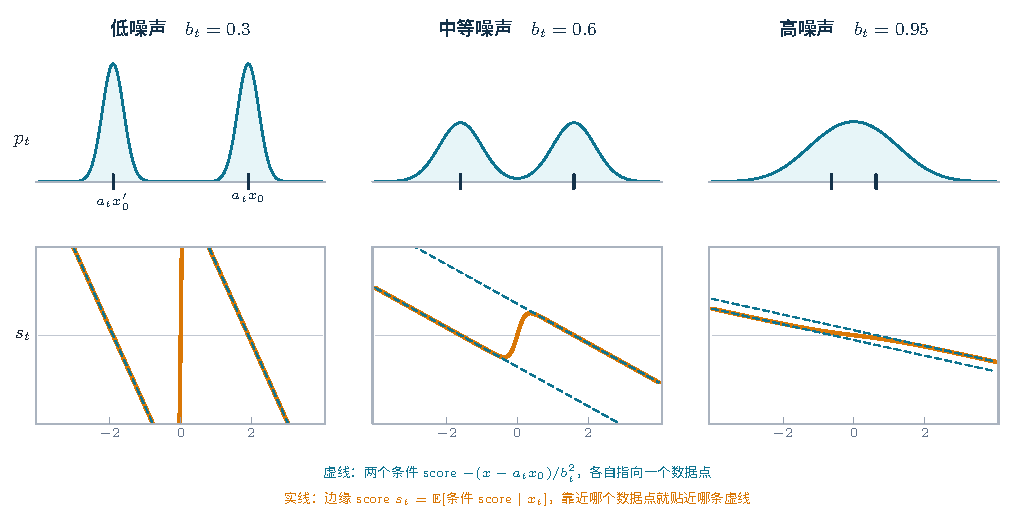
\includegraphics[width=\textwidth]{score_noise_levels.pdf}
\caption{两个数据点在三个噪声水平下的密度与 score。上排是带噪边缘密度 \(p_t\)，竖线标出两个高斯中心 \(a_tx_0,a_tx_0'\)。下排虚线是两个条件 score \(c_t=-(x-a_tx_0)/b_t^2\)，实线是边缘 score \(s_t=\E[c_t\mid x_t]\)，三列纵轴比例相同。低噪声时条件 score 很陡，边缘 score 在两峰之间几乎跳变；中等噪声时过渡变缓；高噪声时两条条件 score 接近重合，边缘 score 几乎是一条直线。去噪网络回归的标签是虚线，学到的是实线。}
\label{fig:score-noise-levels}
\end{figure}

同一网络还可以改为预测干净样本 \(\hat x_0\) 或旋转坐标 \(v=a_t\epsilon-b_tx_0\)，三者满足
\begin{equation}
 \hat x_0=\frac{x_t-b_t\epsilon_\theta}{a_t},\qquad
 \hat x_0=a_tx_t-b_t\hat v,\qquad
 \hat\epsilon=b_tx_t+a_t\hat v.
\end{equation}
这里利用了 \(a_t^2+b_t^2=1\)；这些转换在相应分母非零的时间区间成立。\(v\) 在这里是信号与噪声的旋转坐标；后文 Flow Matching 使用另一个时间变量与速度记号。不同输出参数化若要对应同一个训练目标，还必须相应调整损失权重。

\subsection{从随机扩散到概率流}

为了统一描述加噪步长和采样器，先把离散时间细化到连续时间。随机微分方程（Stochastic Differential Equation，SDE）同时描述确定性漂移和布朗噪声：
\begin{equation}
 dx=f(x,t)\,dt+g(t)\,dW_t.
 \label{eq:forward-sde}
\end{equation}
其中 \(f\) 是确定性的漂移速度，\(g\) 是噪声幅度。可以把 \(W_t\) 理解为连续时间的随机游走。具体地，它是与 \(x\) 同维的标准布朗运动：在长度为 \(\Delta t>0\) 的时间段内，增量 \(\Delta W_t=W_{t+\Delta t}-W_t\sim\mathcal N(0,\Delta t\,I)\)，不重叠时间段的增量相互独立。实际按小步长 \(\Delta t\) 模拟时，上式对应
\begin{equation}
 x_{t+\Delta t}\approx x_t+f(x_t,t)\Delta t+g(t)\sqrt{\Delta t}\,z,
 \qquad z\sim\mathcal N(0,I).
 \label{eq:forward-sde-step}
\end{equation}
每一步重新抽取 \(z\)。例如令 DDPM 的单步噪声方差为 \(\beta(t)\,dt\)，并用 \(\sqrt{1-\beta(t)dt}\approx1-\tfrac12\beta(t)dt\)，得到 \(f(x,t)=-\tfrac12\beta(t)x\)、\(g(t)=\sqrt{\beta(t)}\)。这说明离散 DDPM 的加噪链如何进入连续时间描述。

正向 SDE 从数据分布 \(p_0\) 走向易采样的 \(p_T\)。当 \(g\) 仅依赖时间、密度与系数足够光滑时，反向过程为
\begin{equation}
 dx=[f(x,t)-g(t)^2s_t(x)]\,dt+g(t)\,d\bar W_t,\qquad t:T\to0.
 \label{eq:reverse-sde}
\end{equation}
\(\bar W_t\) 表示沿反向时间抽取的布朗噪声。式中 \(t\) 从 \(T\) 减小到 0，因而 \(dt<0\)，噪声增量的协方差为 \(I|dt|\)。反向漂移中的 score 项可以用一个小时间步看清楚：令 \(h>0\)，已知当前状态 \(x_t=y\)，求更早的 \(x_{t-h}\)。正向短步转移近似为均值 \(x+f(x,t)h\)、协方差 \(g(t)^2hI\) 的高斯核；贝叶斯公式给出
\begin{equation}
 q(x_{t-h}=x\mid x_t=y)\propto p_{t-h}(x)\,q(x_t=y\mid x_{t-h}=x).
 \label{eq:reverse-bayes-step}
\end{equation}
在 \(x\) 接近 \(y\) 处，把 \(\log p_{t-h}(x)\) 作一阶展开，梯度在 \(h\to0\) 时趋于 \(s_t(y)\)。令 \(\delta=x-y\)，将展开式与高斯核相乘并配方，得到
\begin{equation}
\begin{aligned}
 \log q(x_{t-h}=x\mid x_t=y)
 &\simeq C-\frac{\|\delta+f(y,t)h\|^2}{2g(t)^2h}+s_t(y)^\mathsf T\delta\\
 &=C'-\frac{\|\delta-[-f(y,t)+g(t)^2s_t(y)]h\|^2}{2g(t)^2h},
\end{aligned}
 \label{eq:reverse-complete-square}
\end{equation}
其中 \(C,C'\) 不依赖 \(x\)。因此反向一步近似为高斯分布，其均值与协方差是
\begin{equation}
 x_{t-h}\mid x_t=y\ \approx\ \mathcal N\!\left(y+[-f(y,t)+g(t)^2s_t(y)]h,\ g(t)^2hI\right).
 \label{eq:reverse-step-kernel}
\end{equation}
这正是式 \eqref{eq:reverse-sde} 在 \(dt=-h\) 时的一步更新。直观上，在所有可能演化到 \(y\) 的起点中，原本密度较高的起点更可能被选中；\(s_t=\nabla\log p_t\) 给出这项概率修正的方向。

若希望从同一个初始噪声确定性地生成样本，可以寻找具有相同边缘密度的常微分方程。前面已经从噪声网络得到所需的 score；现在把概率密度的扩散写成由速度场驱动的输运。式 \eqref{eq:forward-sde} 对应的福克--普朗克方程是
\begin{align}
 \partial_t p_t
 &=-\nabla\cdot(f p_t)+\tfrac12g(t)^2\Delta p_t\\
 &=-\nabla\cdot\left[\left(f-\tfrac12g(t)^2s_t\right)p_t\right],
 \label{eq:fokker-planck-flow}
\end{align}
第二行使用 \(\nabla p_t=p_ts_t\)。而 ODE \(dx/dt=u_t(x)\) 的密度满足连续性方程 \(\partial_tp_t=-\nabla\cdot(u_tp_t)\)。逐项比较即得概率流 ODE：
\begin{equation}
 \frac{dx}{dt}=u_t(x):=f(x,t)-\tfrac12g(t)^2s_t(x).
 \label{eq:probability-flow}
\end{equation}
因此它与正向 SDE 描述同一族 \(p_t\)；将其从 \(T\) 积分回 0，可用于生成。上面的贝叶斯反向转移也依次经过这族 \(p_t\)。反向 SDE 与反向积分的概率流 ODE 由此具有相同的时间边缘分布，但单条采样轨迹不同。

\Needspace{6\baselineskip}
\textbf{反向扩散与 Langevin：像在哪，不同在哪。}第 \ref{sec:ebm-mcmc} 节的 Langevin 迭代也是“沿 score 走一步，再加高斯噪声”。把 \(-\nabla_xE_\theta\) 记作 score \(s\)，式 \eqref{eq:langevin-step} 写成
\begin{equation}
 x\leftarrow x+\tfrac{\eta}{2}s(x)+\sqrt\eta\,\xi.
\end{equation}
把 \(\epsilon_\theta=-b_ts_t\) 代入式 \eqref{eq:ddpm-reverse-mean}，DDPM 的反向一步变成
\begin{equation}
 x_{t-1}=\frac{x_t+\beta_ts_t(x_t)}{\sqrt{\alpha_t}}+\sigma_tz.
\end{equation}
两者形式相近，却不是同一种算法。取 \(\sigma_t^2\approx\beta_t\)，并只保留 \(\beta_t\) 的一阶项（\(1/\sqrt{\alpha_t}\approx1+\beta_t/2\)），这一步可以拆成两半：
\begin{equation}
 x_{t-1}\approx x_t
 +\underbrace{\tfrac12\beta_t\bigl[x_t+s_t(x_t)\bigr]}_{\text{概率流 ODE 的一步}}
 +\underbrace{\tfrac12\beta_ts_t(x_t)+\sqrt{\beta_t}\,z}_{\eta=\beta_t\text{ 的 Langevin 一步}}.
 \label{eq:ddpm-langevin-split}
\end{equation}
第一项正是式 \eqref{eq:probability-flow} 在 \(f=-\tfrac12\beta x\)、\(g^2=\beta\) 时沿反向时间走的一步，它把分布从 \(p_t\) 推到 \(p_{t-1}\)。第二项是以 \(p_t\) 为目标的 Langevin 一步；按第 \ref{sec:ebm-mcmc} 节的 Fokker--Planck 验证，它让 \(p_t\) 保持不变，只在同一分布内部重新搅动样本。连续时间里，同样的拆分就是反向 SDE 漂移的恒等式
\begin{equation}
 f-g^2s_t=\bigl(f-\tfrac12g^2s_t\bigr)-\tfrac12g^2s_t,
\end{equation}
前一部分是概率流速度，后一部分与噪声 \(g\,d\bar W_t\) 合起来是一段时长为 \(g^2|dt|\) 的 Langevin 动力学。因此，DDPM 的每一步确实含有半步 Langevin，但另一半是 Langevin 没有的输运；整条采样链并不是在某个固定分布上跑 MCMC。表 \ref{tab:langevin-vs-diffusion} 对照了两者。

\begin{table}[H]
\centering\small
\begin{tabularx}{\textwidth}{>{\bfseries}p{20mm} X X}
\toprule
 & Langevin（第 \ref{sec:ebm-mcmc} 节） & DDPM 反向一步\\
\midrule
目标分布 & 一个固定的 \(p\) & 一串分布 \(p_T\to p_{T-1}\to\cdots\to p_0\)\\
用到的 score & 每步相同的 \(\nabla\log p\) & 每步换成当前噪声水平的 \(s_t\)\\
单步的作用 & 保持 \(p\) 不变，样本在 \(p\) 内移动 & 输运半步把 \(p_t\) 变成 \(p_{t-1}\)，Langevin 半步只在 \(p_t\) 内搅动\\
步数 & 要等链混合，事先难以确定 & 由所选时间点固定，走完即得样本\\
多峰分布 & 跨越峰间低密度区可能极慢 & 高噪声时各峰已连成一片，样本随噪声降低逐渐分到各峰\\
误差来源 & 有限步长偏差与未混合 & score 估计误差与时间离散误差\\
\bottomrule
\end{tabularx}
\caption{Langevin 采样与 DDPM 反向采样的对照。}
\label{tab:langevin-vs-diffusion}
\end{table}

多峰一行是两者最实质的差别。Langevin 要在固定的多峰分布里从一个峰走到另一个峰，必须穿过低密度区，等待时间随势垒高度指数增长。反向扩散从近似单峰的 \(p_T\) 出发，此时各峰尚未分开；随着噪声逐级降低，样本由输运项逐渐分配到不同的峰，各峰所得的样本比例由这条分布序列决定，而不靠样本自己越过势垒。

这个拆分也把几种采样器放到同一张图里。只保留输运项，就是确定性的概率流 ODE 采样器；下一小节的 DDIM 可以看作它的一种离散化。只保留 Langevin 项，在每个噪声水平多走若干步、再逐级降低噪声，就是早期 score 模型使用的退火 Langevin 采样~\cite{song2020ncsn}。两项各走一步，就是 DDPM 的反向一步。Song 等人的预测--校正采样器把两部分显式分开：先用反向 SDE 或 ODE 的数值步预测下一噪声水平的样本，再在该水平上做若干步 Langevin 校正~\cite{song2021score}。校正步不改变目标边缘分布，可以减轻数值积分和 score 误差造成的偏离，代价是更多的网络调用。

接下来讨论去噪扩散隐式模型（Denoising Diffusion Implicit Model，DDIM）怎样复用已训练的噪声网络做确定性跳步采样。

\subsection{DDIM：复用噪声网络，改变采样步骤}

先回到 DDPM 的生成程序：在 \(t=T,T-1,\ldots,1\) 的每个时间点调用一次 \(\epsilon_\theta(x_t,t)\)，用式 \eqref{eq:ddpm-reverse-mean} 算当前一步的反向高斯均值，再按式 \eqref{eq:ddpm-sampling-step} 抽样得到 \(x_{t-1}\)。它沿相邻时间点逐步更新，通常要调用网络约 \(T\) 次。要减少调用次数，就需要能直接从当前 \(t\) 更新到选定的更早时间 \(s<t\)。

DDIM 沿用 DDPM 训练时的 \(q(x_t\mid x_0)\)、噪声损失和网络 \(\epsilon_\theta\)，改变生成时连接不同噪声水平的方式~\cite{song2021ddim}。这里先看确定性版本。在当前 \(x_t\) 上调用一次网络，得到噪声预测，并按 \(x_t=a_t\hat x_0+b_t\epsilon_\theta(x_t,t)\) 估计干净图片 \(\hat x_0\)。接着用更早时间 \(s\) 的系数把这两个成分重新组合：
\begin{equation}
 \hat x_0=\frac{x_t-b_t\epsilon_\theta(x_t,t)}{a_t},\qquad
 x_s=a_s\hat x_0+b_s\epsilon_\theta(x_t,t),\quad s<t.
 \label{eq:ddim-update}
\end{equation}
这一更新在一步内从 \(t\) 到达 \(s\)，并沿用当前网络对图像内容与噪声方向的预测。相比之下，DDPM 在每个 \(t\) 只构造到 \(t-1\) 的高斯转移，在中间步另抽一份 \(z\)。确定性 DDIM 的式 \eqref{eq:ddim-update} 在给定初始 \(x_T\) 后不再抽新噪声；两种生成程序使用的是同一套已训练的网络参数。除跳步路径外，噪声水平、网络预条件和数值求解器也会影响采样质量与成本，Karras 等对这些设计做了系统比较~\cite{karras2022edm}。

实际采样时先选一列时间 \(T=t_K>t_{K-1}>\cdots>t_0=0\)，并取 \(a_0=1,b_0=0\)。从 \(x_T\sim\mathcal N(0,I)\) 开始，对每个 \(k=K,\ldots,1\) 令 \(t=t_k,s=t_{k-1}\)，执行一次式 \eqref{eq:ddim-update}。例如原训练调度有 \(T=1000\) 个时间点，生成时只选 \(K=50\) 个更新，就调用网络约 50 次。训练目标和噪声预测不变，改变的是生成时间点与从一个时间点到下一个时间点的更新公式。下一小节介绍常用的 U 形网络（U-Net）与扩散 Transformer（Diffusion Transformer，DiT）。

\subsection{噪声预测网络：U-Net 与 DiT}

前面预测噪声的网络 \(\epsilon_\theta(x_t,t,c)\) 通常采用 U-Net 或 DiT~\cite{peebles2023dit}。扩散模型中的 U-Net 以卷积神经网络（Convolutional Neural Network，CNN）为图像主干：每一级用卷积残差块提取特征，再通过步幅为 2 的卷积把特征图的高和宽减半，并通常增加通道数；恢复路径用插值加卷积或转置卷积把高和宽加倍，把编码路径中相同分辨率的特征通过跳跃连接送来，再用卷积残差块融合。CNN 的下采样扩大感受野，跳跃连接保留细节；一些层还加入自注意力以交换较远位置的信息。DiT 则把带噪图像或潜变量切成 patch 序列，由 Transformer 在 patch 之间交换信息，再投影回噪声预测。

\Needspace{3\baselineskip}
图像扩散也可以先用前述 VAE 式自编码器把图片压缩为连续潜变量，在潜空间逐步去噪，再由解码器还原图片；这减少了去噪网络处理的空间尺寸~\cite{rombach2022ldm}。

网络接收当前时间 \(t\)，\(T\) 决定噪声调度的总步数。一种常见实现先用多种频率的正弦、余弦函数把整数 \(t\) 映射为向量 \(u_t\)，再用一个小型 MLP 计算时间嵌入 \(e_t=\operatorname{MLP}(u_t)\)；图像特征仍由上面的卷积主干处理。U-Net 在各残差块中把 \(e_t\) 投影到特征通道，例如执行 \(h\leftarrow h+W_\ell e_t\)；DiT 可用 \(e_t\) 调节块内自适应归一化的缩放、平移和残差门控。时间输入也可改用对应噪声幅度或对数信噪比。文本等条件 \(c\) 可通过交叉注意力注入，即用当前图像表示查询条件表示。图 \ref{fig:diffusion-denoiser} 把潜空间扩散的流程，以及两种网络中时间与条件的注入位置画在一起。

\begin{figure}[H]
\centering
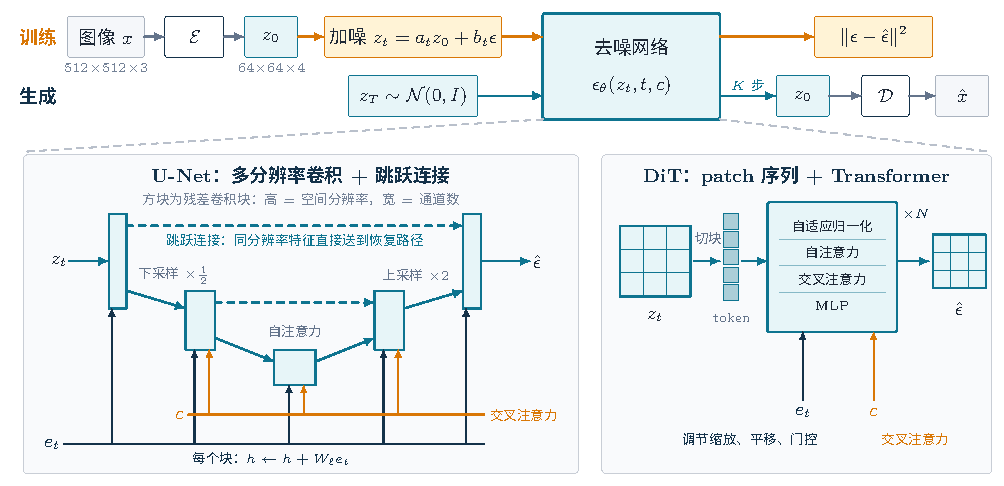
\includegraphics[width=\textwidth]{diffusion_denoiser_arch.pdf}
\caption{潜空间扩散与两种去噪网络。上方：训练时编码器 \(\mathcal E\) 把图像压成潜变量 \(z_0\)，加噪后由网络预测噪声；生成时从 \(z_T\) 出发调用同一网络 \(K\) 步，再由解码器 \(\mathcal D\) 还原图像。左下：U-Net 沿编码路径降低分辨率、增加通道，恢复路径经跳跃连接取回同分辨率特征；时间嵌入 \(e_t\) 加到每个残差块，条件 \(c\) 经交叉注意力进入较低分辨率的块。右下：DiT 把 \(z_t\) 切成 patch token，经 \(N\) 个 Transformer 块后还原为噪声预测；\(e_t\) 调节自适应归一化，\(c\) 经交叉注意力注入。}
\label{fig:diffusion-denoiser}
\end{figure}

当生成还受文本等条件 \(c\) 控制时，常用无分类器引导（classifier-free guidance）增强条件作用。训练时随机把一部分样本的条件替换为空条件，使同一网络既能输出 \(\epsilon_{\mathrm{cond}}=\epsilon_\theta(x_t,t,c)\)，也能输出 \(\epsilon_{\mathrm{uncond}}=\epsilon_\theta(x_t,t,\varnothing)\)。生成时各调用一次网络，将两次预测组合为
\begin{equation}
 \epsilon_{\mathrm{guide}}=\epsilon_{\mathrm{uncond}}+w(\epsilon_{\mathrm{cond}}-\epsilon_{\mathrm{uncond}}).
 \label{eq:cfg}
\end{equation}
\(w=1\) 给出条件预测，\(w>1\) 沿条件与无条件预测之差进一步移动。随后把 \(\epsilon_{\mathrm{guide}}\) 代入 DDPM 或 DDIM 的采样更新；引导改变的是网络给出的更新方向，时间点与采样公式仍由所选采样器决定。按这里分别计算两种预测的做法，每个采样时间需要两次网络调用。

\subsection{Flow Matching：直接学习概率路径的速度}

概率流 ODE 已经把 score 转换成了搬运样本的速度。一个自然的下一步是：能否直接规定从噪声到数据的路径，并把速度当作网络的监督目标？Flow Matching 就采用这一方式~\cite{lipman2023flow}。为与扩散的“数据到噪声”时间区分，本小节用 \(r\in[0,1]\) 表示“噪声到数据”的生成时间。

先看一次训练样本怎样构造。\(y\sim p_{\mathrm{data}}\) 是从数据集中取出的一张真实图片，或它在潜空间中的表示；\(z\sim\mathcal N(0,I)\) 是独立抽取、形状与 \(y\) 相同的高斯噪声。再随机抽 \(r\sim\operatorname{Uniform}[0,1]\)，计算 \(x_r=(1-r)z+ry\)：\(r=0\) 时它是噪声 \(z\)，\(r=1\) 时它是数据 \(y\)。对这一对固定端点，沿 \(r\) 求导得到 \(dx_r/dr=y-z\)；它是从噪声走向真实图片时每单位时间的位移，因而可以直接由已知的 \(y,z\) 算作速度标签。网络 \(v_\theta(x_r,r)\) 接收中间状态和时间，输出与 \(x_r\) 形状相同的预测速度；网络主体也可采用前述 U-Net 或 DiT，并把 \(r\) 作为时间嵌入输入。训练目标是
\begin{equation}
 \mathcal L_{\mathrm{velocity}}
 =\E_{y,z,r}\|v_\theta(x_r,r)-(y-z)\|^2.
 \label{eq:flow-matching}
\end{equation}
实际处理一个大小为 \(B\) 的 minibatch 时，对每张真实图片 \(y_i\) 各抽一个 \(z_i,r_i\)，构造 \(x_{r_i}=(1-r_i)z_i+r_i y_i\) 和标签 \(u_i=y_i-z_i\)。把 \((x_{r_i},r_i)\) 输入网络，逐像素或逐潜变量坐标比较预测速度与 \(u_i\)，再对 batch 取平均：
\begin{equation}
 \widehat{\mathcal L}_{\mathrm{velocity}}=\frac1B\sum_{i=1}^{B}
 \|v_\theta(x_{r_i},r_i)-(y_i-z_i)\|^2.
 \label{eq:flow-matching-batch}
\end{equation}
随后对这个损失反向传播，更新网络参数 \(\theta\)。这里的 \(y_i-z_i\) 是\textbf{速度监督标签}；训练中的梯度是损失对参数 \(\theta\) 的梯度，使网络输出靠近这个标签。在固定 \(x_r=x\) 处，许多不同的 \((y,z)\) 可以产生同一个中间状态，均方回归的最优网络输出是这些速度的条件平均 \(v_r(x)=\E[y-z\mid x_r=x]\)。

这解释了训练标签看似矛盾的地方。网络只看到当前位置与时间，同一输入可能对应多个速度；它在总体均方损失下学到的是这些速度的条件重心。不同的 \(x_r\) 有不同的端点后验，得到的平均速度也不同；生成器沿这个随位置与时间变化的速度场运动。

结论与去噪得分匹配相同：回归条件速度标签，学到的就是搬运边缘分布所需的速度场。理由有两层。第一层是损失本身：与推出式 \eqref{eq:denoising-score} 的正交分解完全相同，在平方中插入 \(v_r(x_r)\) 后交叉项为零，于是
\begin{equation}
 \E\|v_\theta(x_r,r)-(y-z)\|^2
 =\E\|v_\theta(x_r,r)-v_r(x_r)\|^2+C,
 \label{eq:cfm-marginal-equivalence}
\end{equation}
其中 \(C=\E\|(y-z)-v_r(x_r)\|^2\) 是给定 \((x_r,r)\) 后剩余的条件方差，与 \(\theta\) 无关。两种损失的梯度处处相同；\(C>0\) 也说明单对端点的速度有无法从 \((x_r,r)\) 推出的随机部分，训练损失不会降到零。第二层是这个平均速度确实搬运整条概率路径。固定一个数据样本 \(y\) 时，直线上的局部速度是 \(u_r(x\mid y)=(y-x)/(1-r)\)，条件密度 \(p_r(x\mid y)\) 满足连续性方程。对所有 \(y\) 的概率流量求平均，得到
\begin{equation}
 p_r(x)v_r(x)
 =\int p_{\mathrm{data}}(y)\,p_r(x\mid y)\,u_r(x\mid y)\,dy,
 \qquad
 \partial_r p_r(x)+\nabla\cdot\bigl(p_r(x)v_r(x)\bigr)=0.
 \label{eq:flow-matching-marginal-flux}
\end{equation}
第一式是各条条件路径在 \(x\) 处的流量叠加；第二式由条件连续性方程对 \(y\) 积分得到。因此按 \(v_r\) 积分生成 ODE 时，样本在每个 \(r\) 的分布都是训练路径的边缘 \(p_r\)，到 \(r=1\) 就是数据分布；单条生成轨迹与训练用的直线不必相同。

直线路径还给出一个具体图像。在 \(r=0\) 时 \(x_r=z\) 与 \(y\) 独立，所以 \(v_0(x)=\E[y]-x\)。当 \(0<r<1\) 时，由 \(x_r=ry+(1-r)z\) 和高斯噪声得到
\begin{equation}
 p(y\mid x_r=x)\ \propto\ p_{\mathrm{data}}(y)
 \exp\!\left[-\frac{\|x-ry\|^2}{2(1-r)^2}\right].
 \label{eq:flow-matching-endpoint-posterior}
\end{equation}
随着 \(r\) 增大，当前位置对可能的目标数据提供越来越强的约束：不同位置偏向不同的数据区域，速度场便把不同噪声起点引向不同的方向。每一步都会在新的位置重新计算速度，因此这条生成轨迹可以弯曲。

生成新图片时，重新抽一张噪声 \(x^{(0)}=z_{\mathrm{new}}\sim\mathcal N(0,I)\)，选 \(N\) 个时间步 \(r_k=k/N\)、\(\Delta r=1/N\)。每一步用当前状态与时间调用速度网络，再沿预测方向前进一步；最简单的欧拉更新为
\begin{equation}
 x^{(k+1)}=x^{(k)}+\Delta r\,v_\theta(x^{(k)},r_k),
 \qquad k=0,\ldots,N-1.
 \label{eq:flow-matching-euler}
\end{equation}
最后的 \(x^{(N)}\) 就是生成图片。推断时网络只使用当前 \(x^{(k)}\) 与 \(r_k\) 来给出下一步速度；训练所用的真实图片 \(y_i\) 只用于构造监督标签。每对训练端点定义一条直线，条件平均后的速度场可以产生弯曲的生成轨迹。

它与扩散模型的数学关系可以在一般高斯路径上看清。令 \(x_r=a(r)y+b(r)z\)，以 \(p_r\) 表示边缘密度、\(s_r=\nabla\log p_r\)，并在 \(a,b>0\) 的内部时间区间计算。式 \eqref{eq:marginal-score-identity} 给出
\begin{equation}
 \E[z\mid x_r=x]=-b(r)s_r(x),\qquad
 \E[y\mid x_r=x]=\frac{x+b(r)^2s_r(x)}{a(r)}.
\end{equation}
条件速度是 \(\dot a\,y+\dot b\,z\)，点表示对 \(r\) 求导。取条件均值并代入上式得到
\begin{equation}
 v_r(x)=\frac{\dot a}{a}x+
 \left(\frac{\dot a}{a}b^2-b\dot b\right)s_r(x).
 \label{eq:flow-score-bridge}
\end{equation}
式 \eqref{eq:flow-score-bridge} 可以代入两种具体路径。先代入本小节训练用的直线路径 \(a(r)=r,b(r)=1-r\)，此时 \(\dot a=1,\dot b=-1\)，得到
\begin{equation}
 v_r(x)=\E[y-z\mid x_r=x]
 =\frac{x}{r}+\frac{1-r}{r}s_r(x),\qquad 0<r<1.
 \label{eq:straight-flow-score}
\end{equation}
左边正是式 \eqref{eq:flow-matching} 的均方回归在固定 \(x_r=x\) 时学到的速度；右边把同一速度写成了边缘密度的 score。

再代入 DDPM 高斯加噪的连续时间版本。若离散单步方差按 \(\beta_s\approx\beta(t_s)\Delta t\) 缩小，则乘积 \(\bar\alpha_t=\prod_s(1-\beta_s)\) 趋于 \(\bar\alpha(t)=\exp[-\int_0^t\beta(u)\,du]\)。于是正向路径 \(x_t=a(t)y+b(t)z\) 的两个系数为 \(a(t)=\sqrt{\bar\alpha(t)}\)、\(b(t)=\sqrt{1-\bar\alpha(t)}\)。它们满足
\begin{equation}
 \frac{\dot a(t)}{a(t)}=-\frac{\beta(t)}2,\qquad
 b(t)\dot b(t)=\frac{\beta(t)}2a(t)^2,\qquad a(t)^2+b(t)^2=1.
 \label{eq:vp-path-derivatives}
\end{equation}
逐项代入式 \eqref{eq:flow-score-bridge}，便得到
\begin{equation}
\begin{aligned}
 v_t(x)
 &=-\frac{\beta(t)}2x-\frac{\beta(t)}2[b(t)^2+a(t)^2]s_t(x)\\
 &=-\frac{\beta(t)}2x-\frac{\beta(t)}2s_t(x)
 =f(x,t)-\frac12g(t)^2s_t(x),
\end{aligned}
 \label{eq:vp-flow-from-bridge}
\end{equation}
其中 \(f(x,t)=-\beta(t)x/2\)、\(g(t)^2=\beta(t)\)，正是前面 DDPM 连续化得到的漂移和噪声强度。因此同一个一般公式既给出直线 Flow Matching 的最优速度，也给出扩散路径的式 \eqref{eq:probability-flow}。如果 Flow Matching 训练时也选用后一组 \(a(t),b(t)\)，它学到的就是这条扩散路径的概率流速度；本小节先前演示的直线路径则给出另一条速度场。扩散路径的公式按正向时间 \(t\) 表示数据到噪声的速度；生成时从 \(T\) 积分回 0，或改用 \(r=1-t/T\) 并把速度乘以 \(dt/dr=-T\)。这里得到的是确定性的概率流速度，DDPM 的随机反向高斯更新由式 \eqref{eq:ddpm-sampling-step} 给出。

现在可以把第 \ref{sec:cnf} 节的 CNF 与本小节接起来：两者在生成时都从基分布沿 \(dx_r/dr=v_\theta(x_r,r)\) 积分，密度都遵循式 \eqref{eq:cnf-density}。CNF 指这种连续时间的可逆概率变换；Flow Matching 给出学习其速度场的一种监督方法。传统似然训练对每个数据样本求解 ODE 和散度积分，再优化 \(-\log p_1(x)\)；Flow Matching 则先指定具有解析采样公式的条件路径，随机取一个时间和一对端点，直接构造 \(x_r\) 与条件速度标签，按式 \eqref{eq:flow-matching} 回归，训练时不要求解生成 ODE。生成时仍按式 \eqref{eq:flow-matching-euler} 或更精确的求解器积分。若任务需要评价样本密度，也可对训练好的速度场反向积分并累积散度，由 CNF 公式得到 \(\log p_\theta(x)\) 的数值结果。

\begin{table}[H]
\centering\small
\begin{tabularx}{\textwidth}{>{\bfseries}p{28mm} X X}
\toprule
训练方式 & 参数更新时的计算 & 生成与密度评价\\
\midrule
CNF 的似然训练 & 从数据反向求解状态与散度，优化负对数似然 & 积分速度 ODE 生成；积分散度评价密度\\
Flow Matching & 解析构造随机时刻的状态和条件速度，做均方回归 & 积分同类速度 ODE 生成；需要密度时也积分散度\\
\bottomrule
\end{tabularx}
\caption{CNF 的两种训练路径共享连续时间的生成与密度公式。}
\label{tab:cnf-flow-matching}
\end{table}

\begin{figure}[H]
\centering
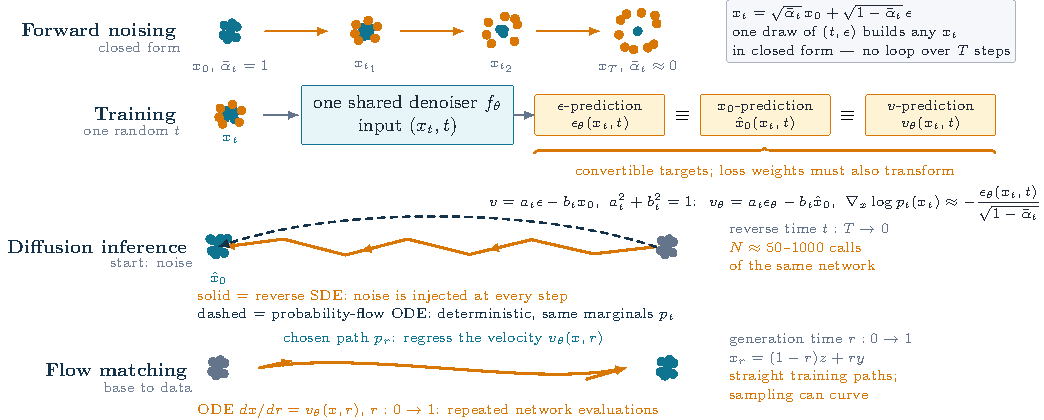
\includegraphics[width=\textwidth]{diffusion_score_flow_paths.pdf}
\caption{训练与生成的四条轨道。正向加噪可直接构造任意时间的训练样本；噪声、干净样本和旋转坐标是可转换的预测对象。扩散采样反向积分 SDE 或概率流 ODE；Flow Matching 用生成时间 \(r\) 直接回归速度并积分。两者通常都需要多次网络调用，相同边缘分布不要求单条轨迹相同。}
\label{fig:diffusion-score}
\end{figure}

\begin{table}[H]
\centering\small
\begin{tabularx}{\textwidth}{>{\bfseries}p{28mm} X X X}
\toprule
方法 & 训练目标 & 生成更新 & 相对 DDPM 的变化\\
\midrule
DDPM & 噪声回归 & 相邻时间的反向高斯转移 & 基线：逐步更新并在中间步抽新噪声\\
连续时间 score & 带噪分布的 score 回归 & 反向 SDE 或概率流 ODE & 用连续时间方向场描述生成\\
确定性 DDIM & 复用 DDPM 的噪声网络 & 从 \(t\) 直接到选定的 \(s<t\) & 由 \(\hat x_0\) 和噪声预测重组，减少网络调用\\
Flow Matching & 所选路径的速度回归 & 从基分布积分速度 ODE & 直接学习速度场，可选择不同概率路径\\
掩码离散扩散 & 被掩码 token 的类别预测及时间加权 & 从全掩码序列逐步恢复 token & 用类别转移代替高斯噪声，可在一轮更新多个位置\\
\bottomrule
\end{tabularx}
\caption{扩散与速度场模型各自改变的数学对象。}
\label{tab:diffusion-score-variants}
\end{table}

\section{模型家族的选择原则}

模型选择的差别可以直接落到任务约束上。下表按模型汇总四件事：它适合什么任务、训练时从哪里得到梯度、推理时沿哪条路径采样、以及代价落在哪里。

\begin{table}[ht]
\centering\scriptsize
\begin{tabularx}{\textwidth}{>{\bfseries}p{19mm} p{26mm} X X X}
\toprule
模型 & 适合的任务约束 & 训练目标与随机性 & 推理路径 & 代价与失效模式\\
\midrule
自回归 & 离散序列、逐步条件控制、需要 token likelihood
& 真实序列 + causal mask，最小化 NLL；训练不需要从模型采样，softmax、注意力和 FFN 全部可微
& 从 BOS 逐 token ancestral sampling，每步读取历史缓存；输入可并行，生成串行
& 串行延迟随输出长度增长；exposure bias；长上下文记忆成本高\\

VAE & 连续数据、需要低维表示和快速重构
& encoder 给 \(q_\phi(z\mid x)\)，decoder 给 \(p_\theta(x\mid z)\)；重参数化，KL 对角高斯时解析
& \(z\sim p(z)\) 后一次 decoder 得到条件分布，再采样 \(x\)；推断时运行 encoder
& 只优化下界；重构偏平滑；强 decoder 会忽略 latent，出现 posterior collapse\\

Flow / RealNVP & 连续数据、需要精确 likelihood、可逆编码或重要性加权
& 变量替换，log-det 解析；训练不需要随机 latent
& \(z\sim p_Z\) 后按逆层一次得到 \(x\)，每层都要反变换
& 可逆结构限制表达；高维 patch、scale 稳定性和多层逆变换带来成本\\

GAN & 单次前向延迟极低、允许隐式分布
& 判别器 BCE 与生成器 minimax 或 non-saturating loss 交替；给定 \(z\)，生成器到判别器的路径可微
& \(z\) 一次过 \(G\)，部署吞吐高
& 无 likelihood；博弈非凸、mode collapse、Nash 均衡难达到\\

Diffusion/\allowbreak Score & 图像或连续场、峰值质量优先、允许多步采样
& 随机抽 \(t,\epsilon\) 构造 \(x_t\)，回归 \(\epsilon\)、\(x_0\)、\(v\) 或 score；普通反传
& 从 \(x_T\) 反复求解 reverse SDE/ODE，\(N_{\mathrm{step}}\) 次网络调用
& 采样成本乘步数；solver、噪声调度和 guidance 改变样本分布\\

EBM & 只知道能量、守恒量或未归一化目标密度
& 正相位降低数据能量，负相位从 \(p_\theta\) 链采样；MCMC 噪声不能直接沿长链反传
& Langevin/MCMC 多步迭代，单步网络便宜但混合可能极慢
& 配分函数和负相位难算；局部链不能代表全局模式\\
\bottomrule
\end{tabularx}
\caption{按模型对照任务约束、训练随机性与梯度路径、推理路径和主要代价。}
\label{tab:model-selection-explicit}
\end{table}

如果任务是“给定前缀继续生成”，自回归模型的优势来自条件分解本身；如果任务是“从噪声一次得到连续样本”，GAN 或 VAE 的单次 decoder 路径更短，但它们对高频细节和分布覆盖的取舍不同。如果必须报告每个样本的 likelihood，GAN 无法给出，VAE 给出 ELBO，可逆流则用变量变换评价密度：RealNVP 显式累加 log-determinant，CNF 数值积分散度。若目标侧重图像感知质量，连续扩散通常以更多采样步换取更稳的多峰覆盖；离散文本也可用掩码扩散逐轮填充，速度与质量需要按具体任务评估。若目标密度由已知能量给出，EBM 的优势是目标写法自然，难点则从表达转移到 MCMC 的负相位和混合。

\section{六类模型的一次实际训练循环}

一次 minibatch 的操作顺序把公式落成可执行计算：从哪一个随机变量、哪一条网络路径和哪一种概率对象算出来。

\subsection{自回归 Transformer}

给定 batch 中的真实序列 \(x_{1:T}\)，先把输入右移一位，形成 \(\langle\mathrm{BOS}\rangle,x_1,\ldots,x_{T-1}\)，经过 embedding、位置编码和 \(L\) 个 decoder block，得到每个位置的 logits \(l_t\)。对真实标签 \(x_t\) 计算
\begin{equation}
\mathcal L_{\mathrm{autoregressive}}=-\frac1T\sum_{t=1}^{T}
\log\operatorname{softmax}(l_t)_{x_t}.
\end{equation}
causal mask 使一次前向同时产生全部 \(T\) 个位置；反向传播更新词向量嵌入、注意力、前馈网络和输出投影。训练时通常只使用 dropout、数据顺序或数据增强中的随机性，不需要从模型的 \(p_\theta\) 采样。推理从 BOS 开始，算出下一个 token 的分布后抽样并追加，再重复运行；历史缓存保存旧 token 已计算的表示，避免每一步重算前缀；具体保存哪些张量将在下一章说明。

\subsection{VAE}

对一个 minibatch 的每个观测 \(x\)，encoder 产生 \(\mu_\phi(x),\log\sigma_\phi^2(x)\)，从独立高斯 \(\epsilon\) 构造 \(z^{(k)}=\mu_\phi(x)+\sigma_\phi(x)\odot\epsilon^{(k)}\)，decoder 产生 \(p_\theta(x\mid z^{(k)})\) 的参数。按式~\eqref{eq:vae-mc-loss} 估计每个 \(x\) 的负 ELBO，再对 minibatch 取平均；标准 VAE 的 KL 系数为 \(1\)，另设系数 \(\beta\neq1\) 时是加权变体。观测 \(x\) 在 decoder 分布下的负对数概率沿 decoder 和重参数化路径更新 \(\theta,\phi\)，KL 项沿 encoder 的 \(\mu,\log\sigma^2\) 更新 \(\phi\)。二值数据的 Bernoulli 选择给出逐位交叉熵；连续数据的固定方差高斯选择给出带尺度的均方误差。生成阶段不需要 encoder：先采样 \(z\sim p(z)\)，再从 decoder 给出的条件分布采样 \(x\)。

\subsection{RealNVP Flow}

给定数据 \(x\)，依次运行每层 coupling transform 得 \(z=f_\theta(x)\)，计算 base log-density 与每层 scale 的和：
\begin{equation}
\mathcal L_{\mathrm{Flow}}
=-\log p_Z(z)-\sum_{\ell}\sum_j s_{\ell,j}(x_{a,\ell}).
\end{equation}
由于正向变换和 log-determinant 都是确定可微的，梯度直接更新每层产生 \(s,t\) 的网络；训练中没有从 \(z\) 采样。部署时从 \(z\sim p_Z\) 开始，按逆序计算 \(x_b=(z_b-t(z_a))e^{-s(z_a)}\)，无需迭代求解。若还要做 importance sampling，可用 exact \(p_X(x)\) 对样本重加权；这正是 Flow 相对 GAN/VAE 的概率优势。

\subsection{生成对抗网络}

一次训练循环包含判别器更新与生成器更新，两步分别使用各自的损失。

每个 discriminator step 取真实 batch \(x\sim p_{\mathrm{data}}\) 和噪声 batch \(z\sim p_Z\)，构造 \(x_g=G_\theta(z)\)，最小化
\begin{equation}
\mathcal L_D=-\E_x\log D_\phi(x)-\E_z\log(1-D_\phi(x_g)).
\end{equation}
随后冻结 \(D\)，重新取噪声或复用 \(x_g\)，最小化
\(\mathcal L_G=-\E_z\log D_\phi(G_\theta(z))\)。判别器的梯度不能更新生成器，生成器的梯度必须通过 \(D(G(z))\) 回到 \(G\)；因此实现上要在两个 optimizer step 之间切换 requires-grad。推理时只保留 \(G\)，每个噪声一次前向得到一个样本；训练的不稳定来自两个网络的相对速度和分布支撑，与采样链无关。

\subsection{Diffusion / Score}

每个训练样本只随机抽一个时间 \(t\) 和一个噪声 \(\epsilon\)，通过
\begin{equation}
x_t=a_tx_0+b_t\epsilon,\qquad a_t=\sqrt{\bar\alpha_t},\quad b_t=\sqrt{1-\bar\alpha_t},
\end{equation}
构造网络输入，计算 \(\|\epsilon-\epsilon_\theta(x_t,t,c)\|^2\)，再标准反向传播。随机噪声不需要对 \(\epsilon\) 求梯度；它只是把同一个 \(x_0\) 变成不同噪声层级的训练实例。推理从 \(x_T\sim\mathcal N(0,I)\) 开始，重复调用同一 denoiser 并使用离散 reverse update、SDE solver 或 probability-flow ODE solver；一次样本需要 \(N_{\mathrm{step}}\) 次网络前向，因此采样成本与步数直接相乘。

\subsection{EBM}

每次更新先用真实数据计算 positive phase，再从当前能量模型的 MCMC 链得到 negative samples，使用
\begin{equation}
\widehat{\nabla_\theta\mathcal L}
=\frac1B\sum_i\nabla_\theta E_\theta(x_i^{+})
-\frac1B\sum_i\nabla_\theta E_\theta(x_i^{-}).
\end{equation}
短链得到的 \(x_i^{-}\) 与真实独立样本有偏差，所以参数更新和采样链互相影响。一个具体的 persistent chain 循环是：初始化并保存 \(M\) 个链状态；每个 minibatch 到来时，从这些旧状态各走 \(k\) 步 Gibbs、Metropolis--Hastings 或 Langevin 更新；用终点估计 negative phase；完成一次参数更新；最后把终点写回状态池，供下一 minibatch 继续。它省掉了每轮从随机初值重新 burn-in，却引入两类偏差：有限 \(k\) 使样本相关，参数在链尚未平衡时已经变化；若能量面有分离很远的模式，链还可能长期困在某一模式。实务中应监控多链能量、模式占比、自相关时间和跨模式跃迁，与训练 loss 一起看。推理阶段也运行同样的链，模型的表达和目标密度写法很灵活，代价集中在负相位和混合。

\begin{table}[H]
\centering\small
\begin{tabularx}{\textwidth}{>{\bfseries}p{26mm} X X X}
\toprule
模型 & 每步抽什么随机量 & 梯度从哪里来 & 推理调用几次网络\\
\midrule
自回归 & 数据顺序、dropout & 词表交叉熵，全部可微 & 每个新 token 一次，读取历史缓存\\
VAE & $\epsilon\sim\mathcal N(0,I)$ & 重参数化路径，KL 解析式 & 一次 decoder\\
RealNVP & 训练时无；生成时 $z\sim p_Z$ & 变量替换，正向与逆变换都可微 & 每层一次逆变换\\
GAN & $z\sim p_Z$ & 经判别器 $D(G(z))$ 回传 & 一次生成器\\
Diffusion & $t,\epsilon$ & 噪声回归，普通反向传播 & $N_{\mathrm{step}}$ 次 denoiser\\
EBM & MCMC 链的状态 & 正负相位，链本身不反传 & 多步 MCMC\\
\bottomrule
\end{tabularx}
\caption{六个训练循环只差三处：每步抽什么随机量、梯度沿哪条路径回传、推理要调用几次网络。}
\label{tab:six-loops}
\end{table}
